\newgeometry{
  top=14mm,
  bottom=11mm,
  right=10mm,
  left=22mm,
}

\begin{landscape}

%\setlength{\headsep}{5.6mm} 
%\setlength{\topmargin}{-27mm}
\setlength{\footskip}{15.5pt}
%\setlength{\textwidth}{305mm}

\color{uniblue}{\section[(справочное) Перечень сигналов ФСУ, предназначенных для \newline конфигурирования устройства <<ЮНИТ-М300-Т>>]{(справочное)\\Перечень сигналов ФСУ, предназначенных для конфигурирования устройства <<ЮНИТ-М300-Т>>}\label{app:signals}}
\color{black}

\begin{enumerate}[label=\ref{app:signals}.\arabic*] % Без глобального влияния
  \item Перечень сигналов самодиагностики, доступных для конфигурирования, приведен в документации ЮТКБ.656122.609 РЭ <<Устройство защиты и автоматики серии <<ЮНИТ-М300>>. Руководство по эксплуатации общее>>.
  \item Условные обозначения, применяемые в таблице перечня сигналов:
  \begin{itemize}
    \item[$\text{(--)}$] { - сигнал не имеет возможности конфигурации;}
    \item[$\text{(+)}$] { - сигнал имеет возможность конфигурации;}
    \item[$\text{(*)}$] { - конфигурация сигнала предустановлена по умолчанию в сервисном ПО <<ЮНИТ-СЕРВИС>> и не может быть изменена.}
  \end{itemize}
\end{enumerate}

\small % сделаем шрифт в таблице поменьше
% В таблице ниже убрал правую и левую горизонтальные линии чтобы не сливались и жирно видно - также в настройках geometry прищлось поле right =8mm а не 5 mm 
% так как строки ниже колонтитулов спускались
\begin{longtable}{
>{\centering\arraybackslash}m{6.0cm}
|>{\centering\arraybackslash}m{3.45cm}
|>{\centering\arraybackslash}m{2cm}
|>{\centering\arraybackslash}m{2cm}
|>{\centering\arraybackslash}m{2cm}
|>{\centering\arraybackslash}m{2cm}
|>{\centering\arraybackslash}m{2cm}
|>{\centering\arraybackslash}m{2cm}
|>{\centering\arraybackslash}m{2.107cm}
}

%\caption{Перечень сигналов ФСУ, предназначенных для конфигурирования устройств ЮНИТ-М300\vspace{-0.5\baselineskip}}\label{appA:tbl1}\\ % выравнивает надпись посередине таблицы
\caption{Перечень сигналов ФСУ, предназначенных для конфигурирования устройства\hfill\vspace{-0.5\baselineskip}}\label{appA:tbl1}\\ 

\hline
\rowcolor{gray!30}
Полное наименование сигнала & Наименование сигнала на ФСУ & Дискретные входы & Выходные реле & Светодиоды & Функционал. клавиши & Регистратор событий & Аварийный осциллограф & Пуск авар. осциллографа \\ 
\hline
\endfirsthead
%\caption{\emph{Продолжение\vspace{-0.5\baselineskip}}} \\ % Отступ обозначения таблицы от таблицы и выравнивание надписи слева
\caption*{\hspace{3pt}\emph{Продолжение таблицы \ref{appA:tbl1}\hfill\vspace{-0.5\baselineskip}}} \\ % сделано по ГОСТ 2.105 п.6.8.7
\hline
\rowcolor{gray!30}
Полное наименование сигнала & Наименование сигнала на ФСУ & Дискретные входы & Выходные реле & Светодиоды & Функционал. клавиши & Регистратор событий & Аварийный осциллограф & Пуск авар. осциллографа \\ 
%\hline
\endhead

%\hline
\endfoot

%\hline
\endlastfoot

%===t2
\multicolumn{9}{c}{\textbf{Виртуальные кнопки}} \\
\hline
\raggedright Возврат АПВН & \centering Возврат ЧАПВ/АПВН & \centering -- & \centering -- & \centering -- & \centering + & \centering + & \centering + & \centering \arraybackslash + \\ \hline
\multicolumn{9}{c}{\textbf{Виртуальные ключи}} \\
\hline
\raggedright Вывод терминала & \centering Вывод терминала & \centering -- & \centering -- & \centering -- & \centering + & \centering + & \centering + & \centering \arraybackslash + \\ \hline
\raggedright Оперативный вывод функции ЗМН & \centering ОВ ЗМН & \centering -- & \centering -- & \centering -- & \centering + & \centering + & \centering + & \centering \arraybackslash + \\ \hline
\raggedright Оперативный вывод 1 ступени ЗМН & \centering ОВ 1 ст. ЗМН & \centering -- & \centering -- & \centering -- & \centering + & \centering + & \centering + & \centering \arraybackslash + \\ \hline
\raggedright Перевод ЗМН 1 ступени на сигнал & \centering ЗМН 1 ст. на сигн & \centering -- & \centering -- & \centering -- & \centering + & \centering + & \centering + & \centering \arraybackslash + \\ \hline
\raggedright Оперативный вывод 2 ступени ЗМН & \centering ОВ 2 ст. ЗМН & \centering -- & \centering -- & \centering -- & \centering + & \centering + & \centering + & \centering \arraybackslash + \\ \hline
\raggedright Перевод ЗМН 2 ступени на сигнал & \centering ЗМН 2 ст. на сигн & \centering -- & \centering -- & \centering -- & \centering + & \centering + & \centering + & \centering \arraybackslash + \\ \hline
\raggedright Оперативный вывод функции ЗФР & \centering ОВ ЗФР & \centering -- & \centering -- & \centering -- & \centering + & \centering + & \centering + & \centering \arraybackslash + \\ \hline
\raggedright Перевод ЗФР на сигнал & \centering ЗФР на сигн & \centering -- & \centering -- & \centering -- & \centering + & \centering + & \centering + & \centering \arraybackslash + \\ \hline
\raggedright Оперативный вывод функции СЗЗ & \centering ОВ СЗЗ & \centering -- & \centering -- & \centering -- & \centering + & \centering + & \centering + & \centering \arraybackslash + \\ \hline
\raggedright Оперативный вывод функции БНН & \centering ОВ БНН & \centering -- & \centering -- & \centering -- & \centering + & \centering + & \centering + & \centering \arraybackslash + \\ \hline
\raggedright Оперативный вывод функции АОСН/АПВН & \centering ОВ АОСН/АПВН & \centering -- & \centering -- & \centering -- & \centering + & \centering + & \centering + & \centering \arraybackslash + \\ \hline
\raggedright Оперативный вывод функции АОСН & \centering ОВ АОСН & \centering -- & \centering -- & \centering -- & \centering + & \centering + & \centering + & \centering \arraybackslash + \\ \hline
\raggedright Оперативный вывод функции АПВН & \centering ОВ АПВН & \centering -- & \centering -- & \centering -- & \centering + & \centering + & \centering + & \centering \arraybackslash + \\ \hline
\raggedright Оперативный вывод функции АОСН1 & \centering ОВ АОСН1 & \centering -- & \centering -- & \centering -- & \centering + & \centering + & \centering + & \centering \arraybackslash + \\ \hline
\raggedright Оперативный вывод функции АОСН2 & \centering ОВ АОСН2 & \centering -- & \centering -- & \centering -- & \centering + & \centering + & \centering + & \centering \arraybackslash + \\ \hline
\raggedright Оперативный вывод функции АОСН3 & \centering ОВ АОСН3 & \centering -- & \centering -- & \centering -- & \centering + & \centering + & \centering + & \centering \arraybackslash + \\ \hline
\raggedright Оперативный вывод функции АПВН1 & \centering ОВ АПВН1 & \centering -- & \centering -- & \centering -- & \centering + & \centering + & \centering + & \centering \arraybackslash + \\ \hline
\raggedright Оперативный вывод функции АПВН2 & \centering ОВ АПВН2 & \centering -- & \centering -- & \centering -- & \centering + & \centering + & \centering + & \centering \arraybackslash + \\ \hline
\raggedright Оперативный вывод функции АПВН3 & \centering ОВ АПВН3 & \centering -- & \centering -- & \centering -- & \centering + & \centering + & \centering + & \centering \arraybackslash + \\ \hline
\raggedright Перевод АОСН1 на сигнал & \centering АОСН1 на сигн & \centering -- & \centering -- & \centering -- & \centering + & \centering + & \centering + & \centering \arraybackslash + \\ \hline
\raggedright Перевод АОСН2 на сигнал & \centering АОСН2 на сигн & \centering -- & \centering -- & \centering -- & \centering + & \centering + & \centering + & \centering \arraybackslash + \\ \hline
\raggedright Перевод АОСН3 на сигнал & \centering АОСН3 на сигн & \centering -- & \centering -- & \centering -- & \centering + & \centering + & \centering + & \centering \arraybackslash + \\ \hline
\raggedright Перевод УВ1 АОСН на сигнал & \centering УВ1 АОСН на сигн & \centering -- & \centering -- & \centering -- & \centering + & \centering + & \centering + & \centering \arraybackslash + \\ \hline
\raggedright Перевод УВ2 АОСН на сигнал & \centering УВ2 АОСН на сигн & \centering -- & \centering -- & \centering -- & \centering + & \centering + & \centering + & \centering \arraybackslash + \\ \hline
\raggedright Перевод УВ3 АОСН на сигнал & \centering УВ3 АОСН на сигн & \centering -- & \centering -- & \centering -- & \centering + & \centering + & \centering + & \centering \arraybackslash + \\ \hline
\raggedright Перевод УВ4 АОСН на сигнал & \centering УВ4 АОСН на сигн & \centering -- & \centering -- & \centering -- & \centering + & \centering + & \centering + & \centering \arraybackslash + \\ \hline
\raggedright Перевод УВ5 АОСН на сигнал & \centering УВ5 АОСН на сигн & \centering -- & \centering -- & \centering -- & \centering + & \centering + & \centering + & \centering \arraybackslash + \\ \hline
\raggedright Перевод УВ6 АОСН на сигнал & \centering УВ6 АОСН на сигн & \centering -- & \centering -- & \centering -- & \centering + & \centering + & \centering + & \centering \arraybackslash + \\ \hline
\raggedright Перевод УВ7 АОСН на сигнал & \centering УВ7 АОСН на сигн & \centering -- & \centering -- & \centering -- & \centering + & \centering + & \centering + & \centering \arraybackslash + \\ \hline
\raggedright Перевод УВ8 АОСН на сигнал & \centering УВ8 АОСН на сигн & \centering -- & \centering -- & \centering -- & \centering + & \centering + & \centering + & \centering \arraybackslash + \\ \hline
\raggedright Перевод УВ9 АОСН на сигнал & \centering УВ9 АОСН на сигн & \centering -- & \centering -- & \centering -- & \centering + & \centering + & \centering + & \centering \arraybackslash + \\ \hline
\raggedright Перевод УВ10 АОСН на сигнал & \centering УВ10 АОСН на сигн & \centering -- & \centering -- & \centering -- & \centering + & \centering + & \centering + & \centering \arraybackslash + \\ \hline
\raggedright Перевод УВ11 АОСН на сигнал & \centering УВ11 АОСН на сигн & \centering -- & \centering -- & \centering -- & \centering + & \centering + & \centering + & \centering \arraybackslash + \\ \hline
\raggedright Перевод УВ12  АОСН на сигнал & \centering УВ12 АОСН на сигн & \centering -- & \centering -- & \centering -- & \centering + & \centering + & \centering + & \centering \arraybackslash + \\ \hline
\raggedright Перевод УВ13 АОСН на сигнал & \centering УВ13 АОСН на сигн & \centering -- & \centering -- & \centering -- & \centering + & \centering + & \centering + & \centering \arraybackslash + \\ \hline
\raggedright Перевод УВ14 АОСН на сигнал & \centering УВ14 АОСН на сигн & \centering -- & \centering -- & \centering -- & \centering + & \centering + & \centering + & \centering \arraybackslash + \\ \hline
\raggedright Перевод УВ15 АОСН на сигнал & \centering УВ15 АОСН на сигн & \centering -- & \centering -- & \centering -- & \centering + & \centering + & \centering + & \centering \arraybackslash + \\ \hline
\raggedright Перевод УВ1 АПВН на сигнал & \centering УВ1 АПВН на сигн & \centering -- & \centering -- & \centering -- & \centering + & \centering + & \centering + & \centering \arraybackslash + \\ \hline
\raggedright Перевод УВ2 АПВН на сигнал & \centering УВ2 АПВН на сигн & \centering -- & \centering -- & \centering -- & \centering + & \centering + & \centering + & \centering \arraybackslash + \\ \hline
\raggedright Перевод УВ3 АПВН на сигнал & \centering УВ3 АПВН на сигн & \centering -- & \centering -- & \centering -- & \centering + & \centering + & \centering + & \centering \arraybackslash + \\ \hline
\raggedright Перевод УВ4 АПВН на сигнал & \centering УВ4 АПВН на сигн & \centering -- & \centering -- & \centering -- & \centering + & \centering + & \centering + & \centering \arraybackslash + \\ \hline
\raggedright Перевод УВ5 АПВН на сигнал & \centering УВ5 АПВН на сигн & \centering -- & \centering -- & \centering -- & \centering + & \centering + & \centering + & \centering \arraybackslash + \\ \hline
\raggedright Перевод УВ6 АПВН на сигнал & \centering УВ6 АПВН на сигн & \centering -- & \centering -- & \centering -- & \centering + & \centering + & \centering + & \centering \arraybackslash + \\ \hline
\raggedright Перевод УВ7 АПВН на сигнал & \centering УВ7 АПВН на сигн & \centering -- & \centering -- & \centering -- & \centering + & \centering + & \centering + & \centering \arraybackslash + \\ \hline
\raggedright Перевод УВ8 АПВН на сигнал & \centering УВ8 АПВН на сигн & \centering -- & \centering -- & \centering -- & \centering + & \centering + & \centering + & \centering \arraybackslash + \\ \hline
\raggedright Перевод УВ9 АПВН на сигнал & \centering УВ9 АПВН на сигн & \centering -- & \centering -- & \centering -- & \centering + & \centering + & \centering + & \centering \arraybackslash + \\ \hline
\raggedright Перевод УВ10 АПВН на сигнал & \centering УВ10 АПВН на сигн & \centering -- & \centering -- & \centering -- & \centering + & \centering + & \centering + & \centering \arraybackslash + \\ \hline
\raggedright Перевод УВ11 АПВН на сигнал & \centering УВ11 АПВН на сигн & \centering -- & \centering -- & \centering -- & \centering + & \centering + & \centering + & \centering \arraybackslash + \\ \hline
\raggedright Перевод УВ12  АПВН на сигнал & \centering УВ12 АПВН на сигн & \centering -- & \centering -- & \centering -- & \centering + & \centering + & \centering + & \centering \arraybackslash + \\ \hline
\raggedright Перевод УВ13 АПВН на сигнал & \centering УВ13 АПВН на сигн & \centering -- & \centering -- & \centering -- & \centering + & \centering + & \centering + & \centering \arraybackslash + \\ \hline
\raggedright Перевод УВ14 АПВН на сигнал & \centering УВ14 АПВН на сигн & \centering -- & \centering -- & \centering -- & \centering + & \centering + & \centering + & \centering \arraybackslash + \\ \hline
\raggedright Перевод УВ15 АПВН на сигнал & \centering УВ15 АПВН на сигн & \centering -- & \centering -- & \centering -- & \centering + & \centering + & \centering + & \centering \arraybackslash + \\ \hline
\raggedright Перевод АПВН1 на сигнал & \centering АПВН1 на сигн & \centering -- & \centering -- & \centering -- & \centering + & \centering + & \centering + & \centering \arraybackslash + \\ \hline
\raggedright Перевод АПВН2 на сигнал & \centering АПВН2 на сигн & \centering -- & \centering -- & \centering -- & \centering + & \centering + & \centering + & \centering \arraybackslash + \\ \hline
\raggedright Перевод АПВН3 на сигнал & \centering АПВН3 на сигн & \centering -- & \centering -- & \centering -- & \centering + & \centering + & \centering + & \centering \arraybackslash + \\ \hline
\raggedright Оперативный вывод функции АОСЧ & \centering ОВ АОСЧ & \centering -- & \centering -- & \centering -- & \centering + & \centering + & \centering + & \centering \arraybackslash + \\ \hline
\raggedright Оперативный вывод функции АЧР & \centering ОВ АЧР & \centering -- & \centering -- & \centering -- & \centering + & \centering + & \centering + & \centering \arraybackslash + \\ \hline
\raggedright Перевод CАЧР на сигнал & \centering САЧР на сигн & \centering -- & \centering -- & \centering -- & \centering + & \centering + & \centering + & \centering \arraybackslash + \\ \hline
\raggedright Перевод АЧР1 1 на сигнал & \centering АЧР1 1 на сигн & \centering -- & \centering -- & \centering -- & \centering + & \centering + & \centering + & \centering \arraybackslash + \\ \hline
\raggedright Перевод АЧР1 2 на сигнал & \centering АЧР1 2 на сигн & \centering -- & \centering -- & \centering -- & \centering + & \centering + & \centering + & \centering \arraybackslash + \\ \hline
\raggedright Перевод АЧР1 3 на сигнал & \centering АЧР1 3 на сигн & \centering -- & \centering -- & \centering -- & \centering + & \centering + & \centering + & \centering \arraybackslash + \\ \hline
\raggedright Перевод АЧР1 4 на сигнал & \centering АЧР1 4 на сигн & \centering -- & \centering -- & \centering -- & \centering + & \centering + & \centering + & \centering \arraybackslash + \\ \hline
\raggedright Перевод АЧР2 1 на сигнал & \centering АЧР2 1 на сигн & \centering -- & \centering -- & \centering -- & \centering + & \centering + & \centering + & \centering \arraybackslash + \\ \hline
\raggedright Перевод АЧР2 2 на сигнал & \centering АЧР2 2 на сигн & \centering -- & \centering -- & \centering -- & \centering + & \centering + & \centering + & \centering \arraybackslash + \\ \hline
\raggedright Перевод АЧР2 3 на сигнал & \centering АЧР2 3 на сигн & \centering -- & \centering -- & \centering -- & \centering + & \centering + & \centering + & \centering \arraybackslash + \\ \hline
\raggedright Перевод АЧР2 4 на сигнал & \centering АЧР2 4 на сигн & \centering -- & \centering -- & \centering -- & \centering + & \centering + & \centering + & \centering \arraybackslash + \\ \hline
\raggedright Оперативный вывод функции ЧАПВ & \centering ОВ ЧАПВ & \centering -- & \centering -- & \centering -- & \centering + & \centering + & \centering + & \centering \arraybackslash + \\ \hline
\raggedright Перевод ЧАПВ1 на сигнал & \centering ЧАПВ1 на сигн & \centering -- & \centering -- & \centering -- & \centering + & \centering + & \centering + & \centering \arraybackslash + \\ \hline
\raggedright Перевод ЧАПВ2 на сигнал & \centering ЧАПВ2 на сигн & \centering -- & \centering -- & \centering -- & \centering + & \centering + & \centering + & \centering \arraybackslash + \\ \hline
\raggedright Перевод ЧАПВ3 на сигнал & \centering ЧАПВ3 на сигн & \centering -- & \centering -- & \centering -- & \centering + & \centering + & \centering + & \centering \arraybackslash + \\ \hline
\raggedright Перевод ЧАПВ4 на сигнал & \centering ЧАПВ4 на сигн & \centering -- & \centering -- & \centering -- & \centering + & \centering + & \centering + & \centering \arraybackslash + \\ \hline
\multicolumn{9}{c}{\textbf{Общие сигналы функциональной логики}} \\
\hline
\rowcolor{gray!15} 
\multicolumn{9}{c}{Защита минимального напряжения (ЗМН)} \\
\hline
\multicolumn{9}{c}{Защита минимального напряжения 1 ступень (ЗМН 1ст.)} \\
\hline
\raggedright  Функция введена в работу & \centering Ввод & \centering -- & \centering + & \centering + & \centering -- & \centering + & \centering + & \centering \arraybackslash + \\ \hline
\raggedright  Функция оперативно выведена из работы & \centering Оперативный вывод & \centering -- & \centering + & \centering + & \centering -- & \centering + & \centering + & \centering \arraybackslash + \\ \hline
\raggedright  Пуск ИО & \centering ИО U< & \centering -- & \centering + & \centering + & \centering -- & \centering + & \centering + & \centering \arraybackslash + \\ \hline
\raggedright  Пуск & \centering Пуск & \centering -- & \centering + & \centering + & \centering -- & \centering + & \centering + & \centering \arraybackslash + \\ \hline
\raggedright  Срабатывание на сигнал & \centering Срабатывание сигн & \centering -- & \centering + & \centering + & \centering -- & \centering + & \centering + & \centering \arraybackslash + \\ \hline
\raggedright  Срабатывание & \centering Срабатывание & \centering -- & \centering + & \centering + & \centering -- & \centering + & \centering + & \centering \arraybackslash + \\ \hline
\multicolumn{9}{c}{Защита минимального напряжения 2 ступень (ЗМН 2ст.)} \\
\hline
\raggedright  Функция введена в работу & \centering Ввод & \centering -- & \centering + & \centering + & \centering -- & \centering + & \centering + & \centering \arraybackslash + \\ \hline
\raggedright  Функция оперативно выведена из работы & \centering Оперативный вывод & \centering -- & \centering + & \centering + & \centering -- & \centering + & \centering + & \centering \arraybackslash + \\ \hline
\raggedright  Пуск ИО & \centering ИО U< & \centering -- & \centering + & \centering + & \centering -- & \centering + & \centering + & \centering \arraybackslash + \\ \hline
\raggedright  Пуск & \centering Пуск & \centering -- & \centering + & \centering + & \centering -- & \centering + & \centering + & \centering \arraybackslash + \\ \hline
\raggedright  Срабатывание на сигнал & \centering Срабатывание сигн & \centering -- & \centering + & \centering + & \centering -- & \centering + & \centering + & \centering \arraybackslash + \\ \hline
\raggedright  Срабатывание & \centering Срабатывание & \centering -- & \centering + & \centering + & \centering -- & \centering + & \centering + & \centering \arraybackslash + \\ \hline
\rowcolor{gray!15} 
\multicolumn{9}{c}{Защита от феррорезонанса (ЗФР)} \\
\hline
\raggedright  Функция введена в работу & \centering Ввод & \centering -- & \centering + & \centering + & \centering -- & \centering + & \centering + & \centering \arraybackslash + \\ \hline
\raggedright  Функция оперативно выведена из работы & \centering Оперативный вывод & \centering -- & \centering + & \centering + & \centering -- & \centering + & \centering + & \centering \arraybackslash + \\ \hline
\raggedright  ИО 3U0> & \centering ИО 3U0> & \centering -- & \centering + & \centering + & \centering -- & \centering + & \centering + & \centering \arraybackslash + \\ \hline
\raggedright  ИО 3U0< & \centering ИО 3U0< & \centering -- & \centering + & \centering + & \centering -- & \centering + & \centering + & \centering \arraybackslash + \\ \hline
\raggedright  Пуск & \centering Пуск & \centering -- & \centering + & \centering + & \centering -- & \centering + & \centering + & \centering \arraybackslash + \\ \hline
\raggedright  Срабатывание на сигнал & \centering Срабатывание сигн & \centering -- & \centering + & \centering + & \centering -- & \centering + & \centering + & \centering \arraybackslash + \\ \hline
\raggedright  Срабатывание & \centering Срабатывание & \centering -- & \centering + & \centering + & \centering -- & \centering + & \centering + & \centering \arraybackslash + \\ \hline
\rowcolor{gray!15} 
\multicolumn{9}{c}{Сигнализация замыкания на землю (СЗЗ)} \\
\hline
\raggedright  Функция введена в работу & \centering Ввод & \centering -- & \centering + & \centering + & \centering -- & \centering + & \centering + & \centering \arraybackslash + \\ \hline
\raggedright  Функция оперативно выведена из работы & \centering Оперативный вывод & \centering -- & \centering + & \centering + & \centering -- & \centering + & \centering + & \centering \arraybackslash + \\ \hline
\raggedright  Пуск ИО напряжения НП 3U0> & \centering ИО 3U0> & \centering -- & \centering + & \centering + & \centering -- & \centering + & \centering + & \centering \arraybackslash + \\ \hline
\raggedright  Пуск СЗЗ & \centering Пуск & \centering -- & \centering + & \centering + & \centering -- & \centering + & \centering + & \centering \arraybackslash + \\ \hline
\raggedright  Срабатывание СЗЗ & \centering Срабатывание & \centering -- & \centering + & \centering + & \centering -- & \centering + & \centering + & \centering \arraybackslash + \\ \hline
\rowcolor{gray!15} 
\multicolumn{9}{c}{Блокировка при неисправности цепей напряжения (БНН)} \\
\hline
\raggedright  Функция введена в работу & \centering Ввод & \centering -- & \centering + & \centering + & \centering -- & \centering + & \centering + & \centering \arraybackslash + \\ \hline
\raggedright  Функция оперативно выведена из работы & \centering Оперативный вывод & \centering -- & \centering + & \centering + & \centering -- & \centering + & \centering + & \centering \arraybackslash + \\ \hline
\raggedright  Срабатывание ИО небаланса по напряжению & \centering ИО dU0 & \centering -- & \centering + & \centering + & \centering -- & \centering + & \centering + & \centering \arraybackslash + \\ \hline
\raggedright  Срабатывание ИО напряжения & \centering ИО U< & \centering -- & \centering + & \centering + & \centering -- & \centering + & \centering + & \centering \arraybackslash + \\ \hline
\raggedright  Срабатывание ИО напряжения ОП & \centering ИО U2> & \centering -- & \centering + & \centering + & \centering -- & \centering + & \centering + & \centering \arraybackslash + \\ \hline
\raggedright  Срабатывание ИО напряжения НП 3 гармоники & \centering ИО 3U03f< & \centering -- & \centering + & \centering + & \centering -- & \centering + & \centering + & \centering \arraybackslash + \\ \hline
\raggedright  Пуск ИО небаланса по напряжению & \centering Пуск dU0 & \centering -- & \centering + & \centering + & \centering -- & \centering + & \centering + & \centering \arraybackslash + \\ \hline
\raggedright  Пуск ИО минимального напряжения & \centering Пуск minU1p & \centering -- & \centering + & \centering + & \centering -- & \centering + & \centering + & \centering \arraybackslash + \\ \hline
\raggedright  Пуск ИО напряжения ОП/минимального напряжения & \centering Пуск U2minU1p & \centering -- & \centering + & \centering + & \centering -- & \centering + & \centering + & \centering \arraybackslash + \\ \hline
\raggedright  Пуск ИО напряжения ОП & \centering Пуск U2> & \centering -- & \centering + & \centering + & \centering -- & \centering + & \centering + & \centering \arraybackslash + \\ \hline
\raggedright  Пуск ИО напряжения НП 3 гармоники & \centering Пуск 3U03f< & \centering -- & \centering + & \centering + & \centering -- & \centering + & \centering + & \centering \arraybackslash + \\ \hline
\raggedright  Секция в работе & \centering Секция в работе & \centering -- & \centering + & \centering + & \centering -- & \centering + & \centering + & \centering \arraybackslash + \\ \hline
\raggedright  Срабатывание автомата одной из вторичных обмоток ТН & \centering АВ ТН откл & \centering -- & \centering + & \centering + & \centering -- & \centering + & \centering + & \centering \arraybackslash + \\ \hline
\raggedright  Неисправность цепей напряжения & \centering Неисправность ЦН & \centering -- & \centering + & \centering + & \centering -- & \centering + & \centering + & \centering \arraybackslash + \\ \hline
\raggedright  Блокировка ЗМН при неисправности ЦН & \centering Блокировка ЗМН & \centering -- & \centering + & \centering + & \centering -- & \centering + & \centering + & \centering \arraybackslash + \\ \hline
\raggedright  Срабатывание БНН & \centering Срабатывание & \centering -- & \centering + & \centering + & \centering -- & \centering + & \centering + & \centering \arraybackslash + \\ \hline
\rowcolor{gray!15} 
\multicolumn{9}{c}{Автоматика ограничения снижения напряжения (АОСН)} \\
\hline
\multicolumn{9}{c}{Автоматика ограничения снижения напряжения 1 очередь (АОСН 1 ст)} \\
\hline
\raggedright  Функция введена в работу & \centering Ввод & \centering -- & \centering + & \centering + & \centering -- & \centering + & \centering + & \centering \arraybackslash + \\ \hline
\raggedright  Функция оперативно выведена из работы & \centering Оперативный вывод & \centering -- & \centering + & \centering + & \centering -- & \centering + & \centering + & \centering \arraybackslash + \\ \hline
\raggedright  Пуск ИО напряжения & \centering ИО U< & \centering -- & \centering + & \centering + & \centering -- & \centering + & \centering + & \centering \arraybackslash + \\ \hline
\raggedright  Пуск ИО напряжения ПП & \centering ИО U1< & \centering -- & \centering + & \centering + & \centering -- & \centering + & \centering + & \centering \arraybackslash + \\ \hline
\raggedright  Пуск ИО напряжения ПП смежной секции & \centering ИО U1см< & \centering -- & \centering + & \centering + & \centering -- & \centering + & \centering + & \centering \arraybackslash + \\ \hline
\raggedright  Пуск ИО напряжения ОП & \centering ИО U2> & \centering -- & \centering + & \centering + & \centering -- & \centering + & \centering + & \centering \arraybackslash + \\ \hline
\raggedright  Пуск ИО частоты & \centering ИО F< & \centering -- & \centering + & \centering + & \centering -- & \centering + & \centering + & \centering \arraybackslash + \\ \hline
\raggedright  Пуск ИО по скорости снижения напряжения & \centering ИО dU/dt & \centering -- & \centering + & \centering + & \centering -- & \centering + & \centering + & \centering \arraybackslash + \\ \hline
\raggedright  Динамическая блокировка АОСН & \centering Динам. блок. & \centering -- & \centering + & \centering + & \centering -- & \centering + & \centering + & \centering \arraybackslash + \\ \hline
\raggedright  Пуск АОСН & \centering Пуск & \centering -- & \centering + & \centering + & \centering -- & \centering + & \centering + & \centering \arraybackslash + \\ \hline
\raggedright  Срабатывание на сигнал & \centering Срабатывание сигн & \centering -- & \centering + & \centering + & \centering -- & \centering + & \centering + & \centering \arraybackslash + \\ \hline
\raggedright  Срабатывание & \centering Срабатывание & \centering -- & \centering + & \centering + & \centering -- & \centering + & \centering + & \centering \arraybackslash + \\ \hline
\multicolumn{9}{c}{Автоматика ограничения снижения напряжения 2 очередь (АОСН 2 ст)} \\
\hline
\raggedright  Функция введена в работу & \centering Ввод & \centering -- & \centering + & \centering + & \centering -- & \centering + & \centering + & \centering \arraybackslash + \\ \hline
\raggedright  Функция оперативно выведена из работы & \centering Оперативный вывод & \centering -- & \centering + & \centering + & \centering -- & \centering + & \centering + & \centering \arraybackslash + \\ \hline
\raggedright  Пуск ИО напряжения & \centering ИО U< & \centering -- & \centering + & \centering + & \centering -- & \centering + & \centering + & \centering \arraybackslash + \\ \hline
\raggedright  Пуск ИО напряжения ПП & \centering ИО U1< & \centering -- & \centering + & \centering + & \centering -- & \centering + & \centering + & \centering \arraybackslash + \\ \hline
\raggedright  Пуск ИО напряжения ПП смежной секции & \centering ИО U1см< & \centering -- & \centering + & \centering + & \centering -- & \centering + & \centering + & \centering \arraybackslash + \\ \hline
\raggedright  Пуск ИО напряжения ОП & \centering ИО U2> & \centering -- & \centering + & \centering + & \centering -- & \centering + & \centering + & \centering \arraybackslash + \\ \hline
\raggedright  Пуск ИО частоты & \centering ИО F< & \centering -- & \centering + & \centering + & \centering -- & \centering + & \centering + & \centering \arraybackslash + \\ \hline
\raggedright  Пуск ИО по скорости снижения напряжения & \centering ИО dU/dt & \centering -- & \centering + & \centering + & \centering -- & \centering + & \centering + & \centering \arraybackslash + \\ \hline
\raggedright  Динамическая блокировка АОСН & \centering Динам. блок. & \centering -- & \centering + & \centering + & \centering -- & \centering + & \centering + & \centering \arraybackslash + \\ \hline
\raggedright  Пуск АОСН & \centering Пуск & \centering -- & \centering + & \centering + & \centering -- & \centering + & \centering + & \centering \arraybackslash + \\ \hline
\raggedright  Срабатывание на сигнал & \centering Срабатывание сигн & \centering -- & \centering + & \centering + & \centering -- & \centering + & \centering + & \centering \arraybackslash + \\ \hline
\raggedright  Срабатывание & \centering Срабатывание & \centering -- & \centering + & \centering + & \centering -- & \centering + & \centering + & \centering \arraybackslash + \\ \hline
\multicolumn{9}{c}{Автоматика ограничения снижения напряжения 3 очередь (АОСН 3 ст)} \\
\hline
\raggedright  Функция введена в работу & \centering Ввод & \centering -- & \centering + & \centering + & \centering -- & \centering + & \centering + & \centering \arraybackslash + \\ \hline
\raggedright  Функция оперативно выведена из работы & \centering Оперативный вывод & \centering -- & \centering + & \centering + & \centering -- & \centering + & \centering + & \centering \arraybackslash + \\ \hline
\raggedright  Пуск ИО напряжения & \centering ИО U< & \centering -- & \centering + & \centering + & \centering -- & \centering + & \centering + & \centering \arraybackslash + \\ \hline
\raggedright  Пуск ИО напряжения ПП & \centering ИО U1< & \centering -- & \centering + & \centering + & \centering -- & \centering + & \centering + & \centering \arraybackslash + \\ \hline
\raggedright  Пуск ИО напряжения ПП смежной секции & \centering ИО U1см< & \centering -- & \centering + & \centering + & \centering -- & \centering + & \centering + & \centering \arraybackslash + \\ \hline
\raggedright  Пуск ИО напряжения ОП & \centering ИО U2> & \centering -- & \centering + & \centering + & \centering -- & \centering + & \centering + & \centering \arraybackslash + \\ \hline
\raggedright  Пуск ИО частоты & \centering ИО F< & \centering -- & \centering + & \centering + & \centering -- & \centering + & \centering + & \centering \arraybackslash + \\ \hline
\raggedright  Пуск ИО по скорости снижения напряжения & \centering ИО dU/dt & \centering -- & \centering + & \centering + & \centering -- & \centering + & \centering + & \centering \arraybackslash + \\ \hline
\raggedright  Динамическая блокировка АОСН & \centering Динам. блок. & \centering -- & \centering + & \centering + & \centering -- & \centering + & \centering + & \centering \arraybackslash + \\ \hline
\raggedright  Пуск АОСН & \centering Пуск & \centering -- & \centering + & \centering + & \centering -- & \centering + & \centering + & \centering \arraybackslash + \\ \hline
\raggedright  Срабатывание на сигнал & \centering Срабатывание сигн & \centering -- & \centering + & \centering + & \centering -- & \centering + & \centering + & \centering \arraybackslash + \\ \hline
\raggedright  Срабатывание & \centering Срабатывание & \centering -- & \centering + & \centering + & \centering -- & \centering + & \centering + & \centering \arraybackslash + \\ \hline
\multicolumn{9}{c}{Управляющее воздействие 1 АОСН (УВ1 АОСН)} \\
\hline
\raggedright  Срабатывание на сигнал & \centering Срабатывание сигн & \centering -- & \centering + & \centering + & \centering -- & \centering + & \centering + & \centering \arraybackslash + \\ \hline
\raggedright  Срабатывание & \centering Срабатывание & \centering -- & \centering + & \centering + & \centering -- & \centering + & \centering + & \centering \arraybackslash + \\ \hline
\multicolumn{9}{c}{Управляющее воздействие 2 АОСН (УВ2 АОСН)} \\
\hline
\raggedright  Срабатывание на сигнал & \centering Срабатывание сигн & \centering -- & \centering + & \centering + & \centering -- & \centering + & \centering + & \centering \arraybackslash + \\ \hline
\raggedright  Срабатывание & \centering Срабатывание & \centering -- & \centering + & \centering + & \centering -- & \centering + & \centering + & \centering \arraybackslash + \\ \hline
\multicolumn{9}{c}{Управляющее воздействие 3 АОСН (УВ3 АОСН)} \\
\hline
\raggedright  Срабатывание на сигнал & \centering Срабатывание сигн & \centering -- & \centering + & \centering + & \centering -- & \centering + & \centering + & \centering \arraybackslash + \\ \hline
\raggedright  Срабатывание & \centering Срабатывание & \centering -- & \centering + & \centering + & \centering -- & \centering + & \centering + & \centering \arraybackslash + \\ \hline
\multicolumn{9}{c}{Управляющее воздействие 4 АОСН (УВ4 АОСН)} \\
\hline
\raggedright  Срабатывание на сигнал & \centering Срабатывание сигн & \centering -- & \centering + & \centering + & \centering -- & \centering + & \centering + & \centering \arraybackslash + \\ \hline
\raggedright  Срабатывание & \centering Срабатывание & \centering -- & \centering + & \centering + & \centering -- & \centering + & \centering + & \centering \arraybackslash + \\ \hline
\multicolumn{9}{c}{Управляющее воздействие 5 АОСН (УВ5 АОСН)} \\
\hline
\raggedright  Срабатывание на сигнал & \centering Срабатывание сигн & \centering -- & \centering + & \centering + & \centering -- & \centering + & \centering + & \centering \arraybackslash + \\ \hline
\raggedright  Срабатывание & \centering Срабатывание & \centering -- & \centering + & \centering + & \centering -- & \centering + & \centering + & \centering \arraybackslash + \\ \hline
\multicolumn{9}{c}{Управляющее воздействие 6 АОСН (УВ6 АОСН)} \\
\hline
\raggedright  Срабатывание на сигнал & \centering Срабатывание сигн & \centering -- & \centering + & \centering + & \centering -- & \centering + & \centering + & \centering \arraybackslash + \\ \hline
\raggedright  Срабатывание & \centering Срабатывание & \centering -- & \centering + & \centering + & \centering -- & \centering + & \centering + & \centering \arraybackslash + \\ \hline
\multicolumn{9}{c}{Управляющее воздействие 7 АОСН (УВ7 АОСН)} \\
\hline
\raggedright  Срабатывание на сигнал & \centering Срабатывание сигн & \centering -- & \centering + & \centering + & \centering -- & \centering + & \centering + & \centering \arraybackslash + \\ \hline
\raggedright  Срабатывание & \centering Срабатывание & \centering -- & \centering + & \centering + & \centering -- & \centering + & \centering + & \centering \arraybackslash + \\ \hline
\multicolumn{9}{c}{Управляющее воздействие 8 АОСН (УВ8 АОСН)} \\
\hline
\raggedright  Срабатывание на сигнал & \centering Срабатывание сигн & \centering -- & \centering + & \centering + & \centering -- & \centering + & \centering + & \centering \arraybackslash + \\ \hline
\raggedright  Срабатывание & \centering Срабатывание & \centering -- & \centering + & \centering + & \centering -- & \centering + & \centering + & \centering \arraybackslash + \\ \hline
\multicolumn{9}{c}{Управляющее воздействие 9 АОСН (УВ9 АОСН)} \\
\hline
\raggedright  Срабатывание на сигнал & \centering Срабатывание сигн & \centering -- & \centering + & \centering + & \centering -- & \centering + & \centering + & \centering \arraybackslash + \\ \hline
\raggedright  Срабатывание & \centering Срабатывание & \centering -- & \centering + & \centering + & \centering -- & \centering + & \centering + & \centering \arraybackslash + \\ \hline
\multicolumn{9}{c}{Управляющее воздействие 10 АОСН (УВ10 АОСН)} \\
\hline
\raggedright  Срабатывание на сигнал & \centering Срабатывание сигн & \centering -- & \centering + & \centering + & \centering -- & \centering + & \centering + & \centering \arraybackslash + \\ \hline
\raggedright  Срабатывание & \centering Срабатывание & \centering -- & \centering + & \centering + & \centering -- & \centering + & \centering + & \centering \arraybackslash + \\ \hline
\multicolumn{9}{c}{Управляющее воздействие 11 АОСН (УВ11 АОСН)} \\
\hline
\raggedright  Срабатывание на сигнал & \centering Срабатывание сигн & \centering -- & \centering + & \centering + & \centering -- & \centering + & \centering + & \centering \arraybackslash + \\ \hline
\raggedright  Срабатывание & \centering Срабатывание & \centering -- & \centering + & \centering + & \centering -- & \centering + & \centering + & \centering \arraybackslash + \\ \hline
\multicolumn{9}{c}{Управляющее воздействие 12 АОСН (УВ12 АОСН)} \\
\hline
\raggedright  Срабатывание на сигнал & \centering Срабатывание сигн & \centering -- & \centering + & \centering + & \centering -- & \centering + & \centering + & \centering \arraybackslash + \\ \hline
\raggedright  Срабатывание & \centering Срабатывание & \centering -- & \centering + & \centering + & \centering -- & \centering + & \centering + & \centering \arraybackslash + \\ \hline
\multicolumn{9}{c}{Управляющее воздействие 13 АОСН (УВ13 АОСН)} \\
\hline
\raggedright  Срабатывание на сигнал & \centering Срабатывание сигн & \centering -- & \centering + & \centering + & \centering -- & \centering + & \centering + & \centering \arraybackslash + \\ \hline
\raggedright  Срабатывание & \centering Срабатывание & \centering -- & \centering + & \centering + & \centering -- & \centering + & \centering + & \centering \arraybackslash + \\ \hline
\multicolumn{9}{c}{Управляющее воздействие 14 АОСН (УВ14 АОСН)} \\
\hline
\raggedright  Срабатывание на сигнал & \centering Срабатывание сигн & \centering -- & \centering + & \centering + & \centering -- & \centering + & \centering + & \centering \arraybackslash + \\ \hline
\raggedright  Срабатывание & \centering Срабатывание & \centering -- & \centering + & \centering + & \centering -- & \centering + & \centering + & \centering \arraybackslash + \\ \hline
\multicolumn{9}{c}{Управляющее воздействие 15 АОСН (УВ15 АОСН)} \\
\hline
\raggedright  Срабатывание на сигнал & \centering Срабатывание сигн & \centering -- & \centering + & \centering + & \centering -- & \centering + & \centering + & \centering \arraybackslash + \\ \hline
\raggedright  Срабатывание & \centering Срабатывание & \centering -- & \centering + & \centering + & \centering -- & \centering + & \centering + & \centering \arraybackslash + \\ \hline
\multicolumn{9}{c}{Автоматическое повторное включение по напряжению ступень 1 (АПВН 1 ст)} \\
\hline
\raggedright  Функция введена в работу & \centering Ввод & \centering -- & \centering + & \centering + & \centering -- & \centering + & \centering + & \centering \arraybackslash + \\ \hline
\raggedright  Функция оперативно выведена из работы & \centering Оперативный вывод & \centering -- & \centering + & \centering + & \centering -- & \centering + & \centering + & \centering \arraybackslash + \\ \hline
\raggedright  Пуск ИО напряжения ПП & \centering ИО U1> & \centering -- & \centering + & \centering + & \centering -- & \centering + & \centering + & \centering \arraybackslash + \\ \hline
\raggedright  Пуск ИО частоты & \centering ИО F< & \centering -- & \centering + & \centering + & \centering -- & \centering + & \centering + & \centering \arraybackslash + \\ \hline
\raggedright  Блокировка от многократных включений & \centering Блок. повт. АПВН1 & \centering -- & \centering + & \centering + & \centering -- & \centering + & \centering + & \centering \arraybackslash + \\ \hline
\raggedright  Разрешение АПВН & \centering Разрешение & \centering -- & \centering + & \centering + & \centering -- & \centering + & \centering + & \centering \arraybackslash + \\ \hline
\raggedright  Динамическая блокировка АПВН & \centering Динам. блок. & \centering -- & \centering + & \centering + & \centering -- & \centering + & \centering + & \centering \arraybackslash + \\ \hline
\raggedright  Пуск АПВН & \centering Пуск & \centering -- & \centering + & \centering + & \centering -- & \centering + & \centering + & \centering \arraybackslash + \\ \hline
\raggedright  Срабатывание на сигнал & \centering Срабатывание сигн & \centering -- & \centering + & \centering + & \centering -- & \centering + & \centering + & \centering \arraybackslash + \\ \hline
\raggedright  Срабатывание & \centering Срабатывание & \centering -- & \centering + & \centering + & \centering -- & \centering + & \centering + & \centering \arraybackslash + \\ \hline
\multicolumn{9}{c}{Автоматическое повторное включение по напряжению ступень 2 (АПВН 2 ст)} \\
\hline
\raggedright  Функция введена в работу & \centering Ввод & \centering -- & \centering + & \centering + & \centering -- & \centering + & \centering + & \centering \arraybackslash + \\ \hline
\raggedright  Функция оперативно выведена из работы & \centering Оперативный вывод & \centering -- & \centering + & \centering + & \centering -- & \centering + & \centering + & \centering \arraybackslash + \\ \hline
\raggedright  Пуск ИО напряжения ПП & \centering ИО U1> & \centering -- & \centering + & \centering + & \centering -- & \centering + & \centering + & \centering \arraybackslash + \\ \hline
\raggedright  Пуск ИО частоты & \centering ИО F< & \centering -- & \centering + & \centering + & \centering -- & \centering + & \centering + & \centering \arraybackslash + \\ \hline
\raggedright  Блокировка от многократных включений & \centering Блок. повт. АПВН2 & \centering -- & \centering + & \centering + & \centering -- & \centering + & \centering + & \centering \arraybackslash + \\ \hline
\raggedright  Разрешение АПВН & \centering Разрешение & \centering -- & \centering + & \centering + & \centering -- & \centering + & \centering + & \centering \arraybackslash + \\ \hline
\raggedright  Динамическая блокировка АПВН & \centering Динам. блок. & \centering -- & \centering + & \centering + & \centering -- & \centering + & \centering + & \centering \arraybackslash + \\ \hline
\raggedright  Пуск АПВН & \centering Пуск & \centering -- & \centering + & \centering + & \centering -- & \centering + & \centering + & \centering \arraybackslash + \\ \hline
\raggedright  Срабатывание на сигнал & \centering Срабатывание сигн & \centering -- & \centering + & \centering + & \centering -- & \centering + & \centering + & \centering \arraybackslash + \\ \hline
\raggedright  Срабатывание & \centering Срабатывание & \centering -- & \centering + & \centering + & \centering -- & \centering + & \centering + & \centering \arraybackslash + \\ \hline
\multicolumn{9}{c}{Автоматическое повторное включение по напряжению ступень 3 (АПВН 3 ст)} \\
\hline
\raggedright  Функция введена в работу & \centering Ввод & \centering -- & \centering + & \centering + & \centering -- & \centering + & \centering + & \centering \arraybackslash + \\ \hline
\raggedright  Функция оперативно выведена из работы & \centering Оперативный вывод & \centering -- & \centering + & \centering + & \centering -- & \centering + & \centering + & \centering \arraybackslash + \\ \hline
\raggedright  Пуск ИО напряжения ПП & \centering ИО U1> & \centering -- & \centering + & \centering + & \centering -- & \centering + & \centering + & \centering \arraybackslash + \\ \hline
\raggedright  Пуск ИО частоты & \centering ИО F< & \centering -- & \centering + & \centering + & \centering -- & \centering + & \centering + & \centering \arraybackslash + \\ \hline
\raggedright  Блокировка от многократных включений & \centering Блок. повт. АПВН3 & \centering -- & \centering + & \centering + & \centering -- & \centering + & \centering + & \centering \arraybackslash + \\ \hline
\raggedright  Разрешение АПВН & \centering Разрешение & \centering -- & \centering + & \centering + & \centering -- & \centering + & \centering + & \centering \arraybackslash + \\ \hline
\raggedright  Динамическая блокировка АПВН & \centering Динам. блок. & \centering -- & \centering + & \centering + & \centering -- & \centering + & \centering + & \centering \arraybackslash + \\ \hline
\raggedright  Пуск АПВН & \centering Пуск & \centering -- & \centering + & \centering + & \centering -- & \centering + & \centering + & \centering \arraybackslash + \\ \hline
\raggedright  Срабатывание на сигнал & \centering Срабатывание сигн & \centering -- & \centering + & \centering + & \centering -- & \centering + & \centering + & \centering \arraybackslash + \\ \hline
\raggedright  Срабатывание & \centering Срабатывание & \centering -- & \centering + & \centering + & \centering -- & \centering + & \centering + & \centering \arraybackslash + \\ \hline
\multicolumn{9}{c}{Управляющее воздействие 1 АПВН (УВ1 АПВН)} \\
\hline
\raggedright  Срабатывание на сигнал & \centering Срабатывание сигн & \centering -- & \centering + & \centering + & \centering -- & \centering + & \centering + & \centering \arraybackslash + \\ \hline
\raggedright  Срабатывание & \centering Срабатывание & \centering -- & \centering + & \centering + & \centering -- & \centering + & \centering + & \centering \arraybackslash + \\ \hline
\multicolumn{9}{c}{Управляющее воздействие 2 АПВН (УВ2 АПВН)} \\
\hline
\raggedright  Срабатывание на сигнал & \centering Срабатывание сигн & \centering -- & \centering + & \centering + & \centering -- & \centering + & \centering + & \centering \arraybackslash + \\ \hline
\raggedright  Срабатывание & \centering Срабатывание & \centering -- & \centering + & \centering + & \centering -- & \centering + & \centering + & \centering \arraybackslash + \\ \hline
\multicolumn{9}{c}{Управляющее воздействие 3 АПВН (УВ3 АПВН)} \\
\hline
\raggedright  Срабатывание на сигнал & \centering Срабатывание сигн & \centering -- & \centering + & \centering + & \centering -- & \centering + & \centering + & \centering \arraybackslash + \\ \hline
\raggedright  Срабатывание & \centering Срабатывание & \centering -- & \centering + & \centering + & \centering -- & \centering + & \centering + & \centering \arraybackslash + \\ \hline
\multicolumn{9}{c}{Управляющее воздействие 4 АПВН (УВ4 АПВН)} \\
\hline
\raggedright  Срабатывание на сигнал & \centering Срабатывание сигн & \centering -- & \centering + & \centering + & \centering -- & \centering + & \centering + & \centering \arraybackslash + \\ \hline
\raggedright  Срабатывание & \centering Срабатывание & \centering -- & \centering + & \centering + & \centering -- & \centering + & \centering + & \centering \arraybackslash + \\ \hline
\multicolumn{9}{c}{Управляющее воздействие 5 АПВН (УВ5 АПВН)} \\
\hline
\raggedright  Срабатывание на сигнал & \centering Срабатывание сигн & \centering -- & \centering + & \centering + & \centering -- & \centering + & \centering + & \centering \arraybackslash + \\ \hline
\raggedright  Срабатывание & \centering Срабатывание & \centering -- & \centering + & \centering + & \centering -- & \centering + & \centering + & \centering \arraybackslash + \\ \hline
\multicolumn{9}{c}{Управляющее воздействие 6 АПВН (УВ6 АПВН)} \\
\hline
\raggedright  Срабатывание на сигнал & \centering Срабатывание сигн & \centering -- & \centering + & \centering + & \centering -- & \centering + & \centering + & \centering \arraybackslash + \\ \hline
\raggedright  Срабатывание & \centering Срабатывание & \centering -- & \centering + & \centering + & \centering -- & \centering + & \centering + & \centering \arraybackslash + \\ \hline
\multicolumn{9}{c}{Управляющее воздействие 7 АПВН (УВ7 АПВН)} \\
\hline
\raggedright  Срабатывание на сигнал & \centering Срабатывание сигн & \centering -- & \centering + & \centering + & \centering -- & \centering + & \centering + & \centering \arraybackslash + \\ \hline
\raggedright  Срабатывание & \centering Срабатывание & \centering -- & \centering + & \centering + & \centering -- & \centering + & \centering + & \centering \arraybackslash + \\ \hline
\multicolumn{9}{c}{Управляющее воздействие 8 АПВН (УВ8 АПВН)} \\
\hline
\raggedright  Срабатывание на сигнал & \centering Срабатывание сигн & \centering -- & \centering + & \centering + & \centering -- & \centering + & \centering + & \centering \arraybackslash + \\ \hline
\raggedright  Срабатывание & \centering Срабатывание & \centering -- & \centering + & \centering + & \centering -- & \centering + & \centering + & \centering \arraybackslash + \\ \hline
\multicolumn{9}{c}{Управляющее воздействие 9 АПВН (УВ9 АПВН)} \\
\hline
\raggedright  Срабатывание на сигнал & \centering Срабатывание сигн & \centering -- & \centering + & \centering + & \centering -- & \centering + & \centering + & \centering \arraybackslash + \\ \hline
\raggedright  Срабатывание & \centering Срабатывание & \centering -- & \centering + & \centering + & \centering -- & \centering + & \centering + & \centering \arraybackslash + \\ \hline
\multicolumn{9}{c}{Управляющее воздействие 10 АПВН (УВ10 АПВН)} \\
\hline
\raggedright  Срабатывание на сигнал & \centering Срабатывание сигн & \centering -- & \centering + & \centering + & \centering -- & \centering + & \centering + & \centering \arraybackslash + \\ \hline
\raggedright  Срабатывание & \centering Срабатывание & \centering -- & \centering + & \centering + & \centering -- & \centering + & \centering + & \centering \arraybackslash + \\ \hline
\multicolumn{9}{c}{Управляющее воздействие 11 АПВН (УВ11 АПВН)} \\
\hline
\raggedright  Срабатывание на сигнал & \centering Срабатывание сигн & \centering -- & \centering + & \centering + & \centering -- & \centering + & \centering + & \centering \arraybackslash + \\ \hline
\raggedright  Срабатывание & \centering Срабатывание & \centering -- & \centering + & \centering + & \centering -- & \centering + & \centering + & \centering \arraybackslash + \\ \hline
\multicolumn{9}{c}{Управляющее воздействие 12 АПВН (УВ12 АПВН)} \\
\hline
\raggedright  Срабатывание на сигнал & \centering Срабатывание сигн & \centering -- & \centering + & \centering + & \centering -- & \centering + & \centering + & \centering \arraybackslash + \\ \hline
\raggedright  Срабатывание & \centering Срабатывание & \centering -- & \centering + & \centering + & \centering -- & \centering + & \centering + & \centering \arraybackslash + \\ \hline
\multicolumn{9}{c}{Управляющее воздействие 13 АПВН (УВ13 АПВН)} \\
\hline
\raggedright  Срабатывание на сигнал & \centering Срабатывание сигн & \centering -- & \centering + & \centering + & \centering -- & \centering + & \centering + & \centering \arraybackslash + \\ \hline
\raggedright  Срабатывание & \centering Срабатывание & \centering -- & \centering + & \centering + & \centering -- & \centering + & \centering + & \centering \arraybackslash + \\ \hline
\multicolumn{9}{c}{Управляющее воздействие 14 АПВН (УВ14 АПВН)} \\
\hline
\raggedright  Срабатывание на сигнал & \centering Срабатывание сигн & \centering -- & \centering + & \centering + & \centering -- & \centering + & \centering + & \centering \arraybackslash + \\ \hline
\raggedright  Срабатывание & \centering Срабатывание & \centering -- & \centering + & \centering + & \centering -- & \centering + & \centering + & \centering \arraybackslash + \\ \hline
\multicolumn{9}{c}{Управляющее воздействие 15 АПВН (УВ15 АПВН)} \\
\hline
\raggedright  Срабатывание на сигнал & \centering Срабатывание сигн & \centering -- & \centering + & \centering + & \centering -- & \centering + & \centering + & \centering \arraybackslash + \\ \hline
\raggedright  Срабатывание & \centering Срабатывание & \centering -- & \centering + & \centering + & \centering -- & \centering + & \centering + & \centering \arraybackslash + \\ \hline
\rowcolor{gray!15} 
\multicolumn{9}{c}{Автоматическое ограничение снижения частоты (АОСЧ)} \\
\hline
\multicolumn{9}{c}{Блокировка по скорости снижения частоты (БССЧ)} \\
\hline
\raggedright  Функция введена в работу & \centering Ввод & \centering -- & \centering + & \centering + & \centering -- & \centering + & \centering + & \centering \arraybackslash + \\ \hline
\raggedright  Пуск ИО скорости снижения частоты & \centering ИО dFосн/dt> & \centering -- & \centering + & \centering + & \centering -- & \centering + & \centering + & \centering \arraybackslash + \\ \hline
\raggedright  Пуск ИО частоты & \centering ИО Fосн> & \centering -- & \centering + & \centering + & \centering -- & \centering + & \centering + & \centering \arraybackslash + \\ \hline
\raggedright  Пуск & \centering Пуск & \centering -- & \centering + & \centering + & \centering -- & \centering + & \centering + & \centering \arraybackslash + \\ \hline
\raggedright  Срабатывание & \centering Срабатывание & \centering -- & \centering + & \centering + & \centering -- & \centering + & \centering + & \centering \arraybackslash + \\ \hline
\multicolumn{9}{c}{Контроль напряжения и частоты смежной секции шин (КССШ)} \\
\hline
\raggedright  Функция введена в работу & \centering Ввод & \centering -- & \centering + & \centering + & \centering -- & \centering + & \centering + & \centering \arraybackslash + \\ \hline
\raggedright  Пуск ИО напряжения смежной секции & \centering ИО Uсм> & \centering -- & \centering + & \centering + & \centering -- & \centering + & \centering + & \centering \arraybackslash + \\ \hline
\raggedright  Пуск ИО частоты смежной секции & \centering ИО Fсм< & \centering -- & \centering + & \centering + & \centering -- & \centering + & \centering + & \centering \arraybackslash + \\ \hline
\raggedright  Срабатывание & \centering Срабатывание & \centering -- & \centering + & \centering + & \centering -- & \centering + & \centering + & \centering \arraybackslash + \\ \hline
\rowcolor{gray!15} 
\multicolumn{9}{c}{Автоматическая частотная разгрузка (АЧР)} \\
\hline
\multicolumn{9}{c}{Специальная очередь автоматической частотной разгрузки (САЧР)} \\
\hline
\raggedright  Функция введена в работу & \centering Ввод & \centering -- & \centering + & \centering + & \centering -- & \centering + & \centering + & \centering \arraybackslash + \\ \hline
\raggedright  Функция оперативно выведена из работы & \centering Оперативный вывод & \centering -- & \centering + & \centering + & \centering -- & \centering + & \centering + & \centering \arraybackslash + \\ \hline
\raggedright  Пуск ИО снижения частоты & \centering ИО F< & \centering -- & \centering + & \centering + & \centering -- & \centering + & \centering + & \centering \arraybackslash + \\ \hline
\raggedright  Пуск ИО снижения частоты ниже 45 Гц & \centering ИО F<45 & \centering -- & \centering + & \centering + & \centering -- & \centering + & \centering + & \centering \arraybackslash + \\ \hline
\raggedright  Пуск ИО снижения напряжения & \centering ИО U< & \centering -- & \centering + & \centering + & \centering -- & \centering + & \centering + & \centering \arraybackslash + \\ \hline
\raggedright  Динамическая блокировка САЧР & \centering Динам. блок. & \centering -- & \centering + & \centering + & \centering -- & \centering + & \centering + & \centering \arraybackslash + \\ \hline
\raggedright  Пуск & \centering Пуск & \centering -- & \centering + & \centering + & \centering -- & \centering + & \centering + & \centering \arraybackslash + \\ \hline
\raggedright  Срабатывание на сигнал & \centering Срабатывание сигн & \centering -- & \centering + & \centering + & \centering -- & \centering + & \centering + & \centering \arraybackslash + \\ \hline
\raggedright  Срабатывание & \centering Срабатывание & \centering -- & \centering + & \centering + & \centering -- & \centering + & \centering + & \centering \arraybackslash + \\ \hline
\multicolumn{9}{c}{Ступень 1 подсистемы АЧР1 (АЧР1 1)} \\
\hline
\raggedright  Функция введена в работу & \centering Ввод & \centering -- & \centering + & \centering + & \centering -- & \centering + & \centering + & \centering \arraybackslash + \\ \hline
\raggedright  Функция оперативно выведена из работы & \centering Оперативный вывод & \centering -- & \centering + & \centering + & \centering -- & \centering + & \centering + & \centering \arraybackslash + \\ \hline
\raggedright  Пуск ИО снижения частоты & \centering ИО F< & \centering -- & \centering + & \centering + & \centering -- & \centering + & \centering + & \centering \arraybackslash + \\ \hline
\raggedright  Пуск ИО снижения частоты ниже 45 Гц & \centering ИО F<45 & \centering -- & \centering + & \centering + & \centering -- & \centering + & \centering + & \centering \arraybackslash + \\ \hline
\raggedright  Пуск ИО снижения напряжения & \centering ИО U< & \centering -- & \centering + & \centering + & \centering -- & \centering + & \centering + & \centering \arraybackslash + \\ \hline
\raggedright  Динамическая блокировка АОСН & \centering Динам. блок. & \centering -- & \centering + & \centering + & \centering -- & \centering + & \centering + & \centering \arraybackslash + \\ \hline
\raggedright  Пуск & \centering Пуск & \centering -- & \centering + & \centering + & \centering -- & \centering + & \centering + & \centering \arraybackslash + \\ \hline
\raggedright  Срабатывание на сигнал & \centering Срабатывание сигн & \centering -- & \centering + & \centering + & \centering -- & \centering + & \centering + & \centering \arraybackslash + \\ \hline
\raggedright  Срабатывание & \centering Срабатывание & \centering -- & \centering + & \centering + & \centering -- & \centering + & \centering + & \centering \arraybackslash + \\ \hline
\multicolumn{9}{c}{Ступень 2 подсистемы АЧР1 (АЧР1 2)} \\
\hline
\raggedright  Функция введена в работу & \centering Ввод & \centering -- & \centering + & \centering + & \centering -- & \centering + & \centering + & \centering \arraybackslash + \\ \hline
\raggedright  Функция оперативно выведена из работы & \centering Оперативный вывод & \centering -- & \centering + & \centering + & \centering -- & \centering + & \centering + & \centering \arraybackslash + \\ \hline
\raggedright  Пуск ИО снижения частоты & \centering ИО F< & \centering -- & \centering + & \centering + & \centering -- & \centering + & \centering + & \centering \arraybackslash + \\ \hline
\raggedright  Пуск ИО снижения частоты ниже 45 Гц & \centering ИО F<45 & \centering -- & \centering + & \centering + & \centering -- & \centering + & \centering + & \centering \arraybackslash + \\ \hline
\raggedright  Пуск ИО снижения напряжения & \centering ИО U< & \centering -- & \centering + & \centering + & \centering -- & \centering + & \centering + & \centering \arraybackslash + \\ \hline
\raggedright  Динамическая блокировка АОСН & \centering Динам. блок. & \centering -- & \centering + & \centering + & \centering -- & \centering + & \centering + & \centering \arraybackslash + \\ \hline
\raggedright  Пуск & \centering Пуск & \centering -- & \centering + & \centering + & \centering -- & \centering + & \centering + & \centering \arraybackslash + \\ \hline
\raggedright  Срабатывание на сигнал & \centering Срабатывание сигн & \centering -- & \centering + & \centering + & \centering -- & \centering + & \centering + & \centering \arraybackslash + \\ \hline
\raggedright  Срабатывание & \centering Срабатывание & \centering -- & \centering + & \centering + & \centering -- & \centering + & \centering + & \centering \arraybackslash + \\ \hline
\multicolumn{9}{c}{Ступень 3 подсистемы АЧР1 (АЧР1 3)} \\
\hline
\raggedright  Функция введена в работу & \centering Ввод & \centering -- & \centering + & \centering + & \centering -- & \centering + & \centering + & \centering \arraybackslash + \\ \hline
\raggedright  Функция оперативно выведена из работы & \centering Оперативный вывод & \centering -- & \centering + & \centering + & \centering -- & \centering + & \centering + & \centering \arraybackslash + \\ \hline
\raggedright  Пуск ИО снижения частоты & \centering ИО F< & \centering -- & \centering + & \centering + & \centering -- & \centering + & \centering + & \centering \arraybackslash + \\ \hline
\raggedright  Пуск ИО снижения частоты ниже 45 Гц & \centering ИО F<45 & \centering -- & \centering + & \centering + & \centering -- & \centering + & \centering + & \centering \arraybackslash + \\ \hline
\raggedright  Пуск ИО снижения напряжения & \centering ИО U< & \centering -- & \centering + & \centering + & \centering -- & \centering + & \centering + & \centering \arraybackslash + \\ \hline
\raggedright  Динамическая блокировка АОСН & \centering Динам. блок. & \centering -- & \centering + & \centering + & \centering -- & \centering + & \centering + & \centering \arraybackslash + \\ \hline
\raggedright  Пуск & \centering Пуск & \centering -- & \centering + & \centering + & \centering -- & \centering + & \centering + & \centering \arraybackslash + \\ \hline
\raggedright  Срабатывание на сигнал & \centering Срабатывание сигн & \centering -- & \centering + & \centering + & \centering -- & \centering + & \centering + & \centering \arraybackslash + \\ \hline
\raggedright  Срабатывание & \centering Срабатывание & \centering -- & \centering + & \centering + & \centering -- & \centering + & \centering + & \centering \arraybackslash + \\ \hline
\multicolumn{9}{c}{Ступень 4 подсистемы АЧР1 (АЧР1 4)} \\
\hline
\raggedright  Функция введена в работу & \centering Ввод & \centering -- & \centering + & \centering + & \centering -- & \centering + & \centering + & \centering \arraybackslash + \\ \hline
\raggedright  Функция оперативно выведена из работы & \centering Оперативный вывод & \centering -- & \centering + & \centering + & \centering -- & \centering + & \centering + & \centering \arraybackslash + \\ \hline
\raggedright  Пуск ИО снижения частоты & \centering ИО F< & \centering -- & \centering + & \centering + & \centering -- & \centering + & \centering + & \centering \arraybackslash + \\ \hline
\raggedright  Пуск ИО снижения частоты ниже 45 Гц & \centering ИО F<45 & \centering -- & \centering + & \centering + & \centering -- & \centering + & \centering + & \centering \arraybackslash + \\ \hline
\raggedright  Пуск ИО снижения напряжения & \centering ИО U< & \centering -- & \centering + & \centering + & \centering -- & \centering + & \centering + & \centering \arraybackslash + \\ \hline
\raggedright  Динамическая блокировка АОСН & \centering Динам. блок. & \centering -- & \centering + & \centering + & \centering -- & \centering + & \centering + & \centering \arraybackslash + \\ \hline
\raggedright  Пуск & \centering Пуск & \centering -- & \centering + & \centering + & \centering -- & \centering + & \centering + & \centering \arraybackslash + \\ \hline
\raggedright  Срабатывание на сигнал & \centering Срабатывание сигн & \centering -- & \centering + & \centering + & \centering -- & \centering + & \centering + & \centering \arraybackslash + \\ \hline
\raggedright  Срабатывание & \centering Срабатывание & \centering -- & \centering + & \centering + & \centering -- & \centering + & \centering + & \centering \arraybackslash + \\ \hline
\multicolumn{9}{c}{Ступень 1 подсистемы АЧР2 (АЧР2 1)} \\
\hline
\raggedright  Функция введена в работу & \centering Ввод & \centering -- & \centering + & \centering + & \centering -- & \centering + & \centering + & \centering \arraybackslash + \\ \hline
\raggedright  Функция оперативно выведена из работы & \centering Оперативный вывод & \centering -- & \centering + & \centering + & \centering -- & \centering + & \centering + & \centering \arraybackslash + \\ \hline
\raggedright  Пуск ИО снижения частоты & \centering ИО F< & \centering -- & \centering + & \centering + & \centering -- & \centering + & \centering + & \centering \arraybackslash + \\ \hline
\raggedright  Пуск ИО снижения частоты ниже 45 Гц & \centering ИО F<45 & \centering -- & \centering + & \centering + & \centering -- & \centering + & \centering + & \centering \arraybackslash + \\ \hline
\raggedright  Пуск ИО снижения напряжения & \centering ИО U< & \centering -- & \centering + & \centering + & \centering -- & \centering + & \centering + & \centering \arraybackslash + \\ \hline
\raggedright  Динамическая блокировка АОСН & \centering Динам. блок. & \centering -- & \centering + & \centering + & \centering -- & \centering + & \centering + & \centering \arraybackslash + \\ \hline
\raggedright  Пуск & \centering Пуск & \centering -- & \centering + & \centering + & \centering -- & \centering + & \centering + & \centering \arraybackslash + \\ \hline
\raggedright  Срабатывание на сигнал & \centering Срабатывание сигн & \centering -- & \centering + & \centering + & \centering -- & \centering + & \centering + & \centering \arraybackslash + \\ \hline
\raggedright  Срабатывание & \centering Срабатывание & \centering -- & \centering + & \centering + & \centering -- & \centering + & \centering + & \centering \arraybackslash + \\ \hline
\multicolumn{9}{c}{Ступень 2 подсистемы АЧР2 (АЧР2 2)} \\
\hline
\raggedright  Функция введена в работу & \centering Ввод & \centering -- & \centering + & \centering + & \centering -- & \centering + & \centering + & \centering \arraybackslash + \\ \hline
\raggedright  Функция оперативно выведена из работы & \centering Оперативный вывод & \centering -- & \centering + & \centering + & \centering -- & \centering + & \centering + & \centering \arraybackslash + \\ \hline
\raggedright  Пуск ИО снижения частоты & \centering ИО F< & \centering -- & \centering + & \centering + & \centering -- & \centering + & \centering + & \centering \arraybackslash + \\ \hline
\raggedright  Пуск ИО снижения частоты ниже 45 Гц & \centering ИО F<45 & \centering -- & \centering + & \centering + & \centering -- & \centering + & \centering + & \centering \arraybackslash + \\ \hline
\raggedright  Пуск ИО снижения напряжения & \centering ИО U< & \centering -- & \centering + & \centering + & \centering -- & \centering + & \centering + & \centering \arraybackslash + \\ \hline
\raggedright  Динамическая блокировка АОСН & \centering Динам. блок. & \centering -- & \centering + & \centering + & \centering -- & \centering + & \centering + & \centering \arraybackslash + \\ \hline
\raggedright  Пуск & \centering Пуск & \centering -- & \centering + & \centering + & \centering -- & \centering + & \centering + & \centering \arraybackslash + \\ \hline
\raggedright  Срабатывание на сигнал & \centering Срабатывание сигн & \centering -- & \centering + & \centering + & \centering -- & \centering + & \centering + & \centering \arraybackslash + \\ \hline
\raggedright  Срабатывание & \centering Срабатывание & \centering -- & \centering + & \centering + & \centering -- & \centering + & \centering + & \centering \arraybackslash + \\ \hline
\multicolumn{9}{c}{Ступень 3 подсистемы АЧР2 (АЧР2 3)} \\
\hline
\raggedright  Функция введена в работу & \centering Ввод & \centering -- & \centering + & \centering + & \centering -- & \centering + & \centering + & \centering \arraybackslash + \\ \hline
\raggedright  Функция оперативно выведена из работы & \centering Оперативный вывод & \centering -- & \centering + & \centering + & \centering -- & \centering + & \centering + & \centering \arraybackslash + \\ \hline
\raggedright  Пуск ИО снижения частоты & \centering ИО F< & \centering -- & \centering + & \centering + & \centering -- & \centering + & \centering + & \centering \arraybackslash + \\ \hline
\raggedright  Пуск ИО снижения частоты ниже 45 Гц & \centering ИО F<45 & \centering -- & \centering + & \centering + & \centering -- & \centering + & \centering + & \centering \arraybackslash + \\ \hline
\raggedright  Пуск ИО снижения напряжения & \centering ИО U< & \centering -- & \centering + & \centering + & \centering -- & \centering + & \centering + & \centering \arraybackslash + \\ \hline
\raggedright  Динамическая блокировка АОСН & \centering Динам. блок. & \centering -- & \centering + & \centering + & \centering -- & \centering + & \centering + & \centering \arraybackslash + \\ \hline
\raggedright  Пуск & \centering Пуск & \centering -- & \centering + & \centering + & \centering -- & \centering + & \centering + & \centering \arraybackslash + \\ \hline
\raggedright  Срабатывание на сигнал & \centering Срабатывание сигн & \centering -- & \centering + & \centering + & \centering -- & \centering + & \centering + & \centering \arraybackslash + \\ \hline
\raggedright  Срабатывание & \centering Срабатывание & \centering -- & \centering + & \centering + & \centering -- & \centering + & \centering + & \centering \arraybackslash + \\ \hline
\multicolumn{9}{c}{Ступень 4 подсистемы АЧР2 (АЧР2 4)} \\
\hline
\raggedright  Функция введена в работу & \centering Ввод & \centering -- & \centering + & \centering + & \centering -- & \centering + & \centering + & \centering \arraybackslash + \\ \hline
\raggedright  Функция оперативно выведена из работы & \centering Оперативный вывод & \centering -- & \centering + & \centering + & \centering -- & \centering + & \centering + & \centering \arraybackslash + \\ \hline
\raggedright  Пуск ИО снижения частоты & \centering ИО F< & \centering -- & \centering + & \centering + & \centering -- & \centering + & \centering + & \centering \arraybackslash + \\ \hline
\raggedright  Пуск ИО снижения частоты ниже 45 Гц & \centering ИО F<45 & \centering -- & \centering + & \centering + & \centering -- & \centering + & \centering + & \centering \arraybackslash + \\ \hline
\raggedright  Пуск ИО снижения напряжения & \centering ИО U< & \centering -- & \centering + & \centering + & \centering -- & \centering + & \centering + & \centering \arraybackslash + \\ \hline
\raggedright  Динамическая блокировка АОСН & \centering Динам. блок. & \centering -- & \centering + & \centering + & \centering -- & \centering + & \centering + & \centering \arraybackslash + \\ \hline
\raggedright  Пуск & \centering Пуск & \centering -- & \centering + & \centering + & \centering -- & \centering + & \centering + & \centering \arraybackslash + \\ \hline
\raggedright  Срабатывание на сигнал & \centering Срабатывание сигн & \centering -- & \centering + & \centering + & \centering -- & \centering + & \centering + & \centering \arraybackslash + \\ \hline
\raggedright  Срабатывание & \centering Срабатывание & \centering -- & \centering + & \centering + & \centering -- & \centering + & \centering + & \centering \arraybackslash + \\ \hline
\multicolumn{9}{c}{Общие сигналы АЧР (АЧРобщ)} \\
\hline
\raggedright  Срабатывание АЧРобщ & \centering Срабатывание & \centering -- & \centering + & \centering + & \centering -- & \centering + & \centering + & \centering \arraybackslash + \\ \hline
\rowcolor{gray!15} 
\multicolumn{9}{c}{Частотное автоматическое повторное включение (ЧАПВ)} \\
\hline
\multicolumn{9}{c}{Ступень 1 ЧАПВ (ЧАПВ1)} \\
\hline
\raggedright  Функция введена в работу & \centering Ввод & \centering -- & \centering + & \centering + & \centering -- & \centering + & \centering + & \centering \arraybackslash + \\ \hline
\raggedright  Функция оперативно выведена из работы & \centering Оперативный вывод & \centering -- & \centering + & \centering + & \centering -- & \centering + & \centering + & \centering \arraybackslash + \\ \hline
\raggedright  Пуск ИО увеличения частоты & \centering ИО F> & \centering -- & \centering + & \centering + & \centering -- & \centering + & \centering + & \centering \arraybackslash + \\ \hline
\raggedright  Пуск ИО снижения напряжения & \centering ИО U< & \centering -- & \centering + & \centering + & \centering -- & \centering + & \centering + & \centering \arraybackslash + \\ \hline
\raggedright  Блокировка от многократных включений & \centering Блок. повт. ЧАПВ1 & \centering -- & \centering + & \centering + & \centering -- & \centering + & \centering + & \centering \arraybackslash + \\ \hline
\raggedright  Разрешение ЧАПВ & \centering Разрешение & \centering -- & \centering + & \centering + & \centering -- & \centering + & \centering + & \centering \arraybackslash + \\ \hline
\raggedright  Динамическая блокировка ЧАПВ & \centering Динам. блок. & \centering -- & \centering + & \centering + & \centering -- & \centering + & \centering + & \centering \arraybackslash + \\ \hline
\raggedright  Пуск & \centering Пуск & \centering -- & \centering + & \centering + & \centering -- & \centering + & \centering + & \centering \arraybackslash + \\ \hline
\raggedright  Срабатывание на сигнал & \centering Срабатывание сигн & \centering -- & \centering + & \centering + & \centering -- & \centering + & \centering + & \centering \arraybackslash + \\ \hline
\raggedright  Срабатывание & \centering Срабатывание & \centering -- & \centering + & \centering + & \centering -- & \centering + & \centering + & \centering \arraybackslash + \\ \hline
\multicolumn{9}{c}{Ступень 2 ЧАПВ (ЧАПВ2)} \\
\hline
\raggedright  Функция введена в работу & \centering Ввод & \centering -- & \centering + & \centering + & \centering -- & \centering + & \centering + & \centering \arraybackslash + \\ \hline
\raggedright  Функция оперативно выведена из работы & \centering Оперативный вывод & \centering -- & \centering + & \centering + & \centering -- & \centering + & \centering + & \centering \arraybackslash + \\ \hline
\raggedright  Пуск ИО увеличения частоты & \centering ИО F> & \centering -- & \centering + & \centering + & \centering -- & \centering + & \centering + & \centering \arraybackslash + \\ \hline
\raggedright  Пуск ИО снижения напряжения & \centering ИО U< & \centering -- & \centering + & \centering + & \centering -- & \centering + & \centering + & \centering \arraybackslash + \\ \hline
\raggedright  Блокировка от многократных включений & \centering Блок. повт. ЧАПВ2 & \centering -- & \centering + & \centering + & \centering -- & \centering + & \centering + & \centering \arraybackslash + \\ \hline
\raggedright  Разрешение ЧАПВ & \centering Разрешение & \centering -- & \centering + & \centering + & \centering -- & \centering + & \centering + & \centering \arraybackslash + \\ \hline
\raggedright  Динамическая блокировка ЧАПВ & \centering Динам. блок. & \centering -- & \centering + & \centering + & \centering -- & \centering + & \centering + & \centering \arraybackslash + \\ \hline
\raggedright  Пуск & \centering Пуск & \centering -- & \centering + & \centering + & \centering -- & \centering + & \centering + & \centering \arraybackslash + \\ \hline
\raggedright  Срабатывание на сигнал & \centering Срабатывание сигн & \centering -- & \centering + & \centering + & \centering -- & \centering + & \centering + & \centering \arraybackslash + \\ \hline
\raggedright  Срабатывание & \centering Срабатывание & \centering -- & \centering + & \centering + & \centering -- & \centering + & \centering + & \centering \arraybackslash + \\ \hline
\multicolumn{9}{c}{Ступень 3 ЧАПВ (ЧАПВ3)} \\
\hline
\raggedright  Функция введена в работу & \centering Ввод & \centering -- & \centering + & \centering + & \centering -- & \centering + & \centering + & \centering \arraybackslash + \\ \hline
\raggedright  Функция оперативно выведена из работы & \centering Оперативный вывод & \centering -- & \centering + & \centering + & \centering -- & \centering + & \centering + & \centering \arraybackslash + \\ \hline
\raggedright  Пуск ИО увеличения частоты & \centering ИО F> & \centering -- & \centering + & \centering + & \centering -- & \centering + & \centering + & \centering \arraybackslash + \\ \hline
\raggedright  Пуск ИО снижения напряжения & \centering ИО U< & \centering -- & \centering + & \centering + & \centering -- & \centering + & \centering + & \centering \arraybackslash + \\ \hline
\raggedright  Блокировка от многократных включений & \centering Блок. повт. ЧАПВ3 & \centering -- & \centering + & \centering + & \centering -- & \centering + & \centering + & \centering \arraybackslash + \\ \hline
\raggedright  Разрешение ЧАПВ & \centering Разрешение & \centering -- & \centering + & \centering + & \centering -- & \centering + & \centering + & \centering \arraybackslash + \\ \hline
\raggedright  Динамическая блокировка ЧАПВ & \centering Динам. блок. & \centering -- & \centering + & \centering + & \centering -- & \centering + & \centering + & \centering \arraybackslash + \\ \hline
\raggedright  Пуск & \centering Пуск & \centering -- & \centering + & \centering + & \centering -- & \centering + & \centering + & \centering \arraybackslash + \\ \hline
\raggedright  Срабатывание на сигнал & \centering Срабатывание сигн & \centering -- & \centering + & \centering + & \centering -- & \centering + & \centering + & \centering \arraybackslash + \\ \hline
\raggedright  Срабатывание & \centering Срабатывание & \centering -- & \centering + & \centering + & \centering -- & \centering + & \centering + & \centering \arraybackslash + \\ \hline
\multicolumn{9}{c}{Ступень 4 ЧАПВ (ЧАПВ4)} \\
\hline
\raggedright  Функция введена в работу & \centering Ввод & \centering -- & \centering + & \centering + & \centering -- & \centering + & \centering + & \centering \arraybackslash + \\ \hline
\raggedright  Функция оперативно выведена из работы & \centering Оперативный вывод & \centering -- & \centering + & \centering + & \centering -- & \centering + & \centering + & \centering \arraybackslash + \\ \hline
\raggedright  Пуск ИО увеличения частоты & \centering ИО F> & \centering -- & \centering + & \centering + & \centering -- & \centering + & \centering + & \centering \arraybackslash + \\ \hline
\raggedright  Пуск ИО снижения напряжения & \centering ИО U< & \centering -- & \centering + & \centering + & \centering -- & \centering + & \centering + & \centering \arraybackslash + \\ \hline
\raggedright  Блокировка от многократных включений & \centering Блок. повт. ЧАПВ4 & \centering -- & \centering + & \centering + & \centering -- & \centering + & \centering + & \centering \arraybackslash + \\ \hline
\raggedright  Разрешение ЧАПВ & \centering Разрешение & \centering -- & \centering + & \centering + & \centering -- & \centering + & \centering + & \centering \arraybackslash + \\ \hline
\raggedright  Динамическая блокировка ЧАПВ & \centering Динам. блок. & \centering -- & \centering + & \centering + & \centering -- & \centering + & \centering + & \centering \arraybackslash + \\ \hline
\raggedright  Пуск & \centering Пуск & \centering -- & \centering + & \centering + & \centering -- & \centering + & \centering + & \centering \arraybackslash + \\ \hline
\raggedright  Срабатывание на сигнал & \centering Срабатывание сигн & \centering -- & \centering + & \centering + & \centering -- & \centering + & \centering + & \centering \arraybackslash + \\ \hline
\raggedright  Срабатывание & \centering Срабатывание & \centering -- & \centering + & \centering + & \centering -- & \centering + & \centering + & \centering \arraybackslash + \\ \hline
\multicolumn{9}{c}{Общие сигналы ЧАПВ (ЧАПВобщ)} \\
\hline
\raggedright  Срабатывание ЧАПВобщ & \centering Срабатывание & \centering -- & \centering + & \centering + & \centering -- & \centering + & \centering + & \centering \arraybackslash + \\ \hline
\multicolumn{9}{c}{\textbf{Диагностические сигналы модулей в составе устройства}} \\
\hline
\rowcolor{gray!15} 
\multicolumn{9}{c}{{Слот М1. Модуль питания (P02c)}} \\
\hline
\raggedright Критическая неисправность 12 В & \centering Слот М1. Крит. неисправность 12 В & \centering -- & \centering -- & \centering + & \centering -- & \centering + & \centering + & \centering \arraybackslash + \\ \hline 
\raggedright Некритическая неисправность 12 В & \centering Слот М1. Некрит. неисправность 12 В & \centering -- & \centering -- & \centering + & \centering -- & \centering + & \centering + & \centering \arraybackslash + \\ \hline 
\raggedright Критическая неисправность внешнего питания & \centering Слот М1. Крит. неисправность внешнего питания & \centering -- & \centering -- & \centering + & \centering -- & \centering + & \centering + & \centering \arraybackslash + \\ \hline 
\raggedright Некритическая неисправность внешнего питания & \centering Слот М1. Некрит. неисправность внешнего питания & \centering -- & \centering -- & \centering + & \centering -- & \centering + & \centering + & \centering \arraybackslash + \\ \hline 
\raggedright Критическая неисправность модуля питания & \centering Слот М1. Крит. неисправность модуля питания & \centering -- & \centering -- & \centering + & \centering -- & \centering + & \centering + & \centering \arraybackslash + \\ \hline 
\raggedright Некритическая неисправность модуля питания & \centering Слот М1. Некрит. неисправность модуля питания & \centering -- & \centering -- & \centering + & \centering -- & \centering + & \centering + & \centering \arraybackslash + \\ \hline 
\raggedright Несимметрия внешнего питания & \centering Слот М1. Несимметрия питания & \centering -- & \centering -- & \centering + & \centering -- & \centering + & \centering + & \centering \arraybackslash + \\ \hline 
\raggedright Перегрузка по питанию & \centering Слот М1. Перегрузка по питанию & \centering -- & \centering -- & \centering + & \centering -- & \centering + & \centering + & \centering \arraybackslash + \\ \hline 
\raggedright Неисправность АЦП & \centering Слот М1. Неисправность АЦП & \centering -- & \centering -- & \centering + & \centering -- & \centering + & \centering + & \centering \arraybackslash + \\ \hline 
\raggedright Статус сигнального реле & \centering Слот М1. Статус сигнального реле & \centering -- & \centering -- & \centering + & \centering -- & \centering + & \centering + & \centering \arraybackslash + \\ \hline 
\raggedright Статус светодиода «Готовность» & \centering Слот М1. Статус светодиода «Готовность» & \centering -- & \centering -- & \centering + & \centering -- & \centering + & \centering + & \centering \arraybackslash + \\ \hline 
\raggedright Статус светодиода «Тест» & \centering Слот М1. Статус светодиода «Тест» & \centering -- & \centering -- & \centering + & \centering -- & \centering + & \centering + & \centering \arraybackslash + \\ \hline 
\raggedright Статус сигнализации «Неисправность» & \centering Слот М1. Статус сигнализации «Неисправность» & \centering -- & \centering -- & \centering + & \centering -- & \centering + & \centering + & \centering \arraybackslash + \\ \hline 
\raggedright Статус входа PPS & \centering Слот М1. Статус входа PPS & \centering -- & \centering -- & \centering + & \centering -- & \centering + & \centering + & \centering \arraybackslash + \\ \hline 
\raggedright Наличие внешнего питания & \centering Слот М1. Наличие внешнего питания & \centering -- & \centering -- & \centering + & \centering -- & \centering + & \centering + & \centering \arraybackslash + \\ \hline 
\raggedright Внутренняя неисправность & \centering Слот М1. Внутренняя неисправность & \centering -- & \centering -- & \centering + & \centering -- & \centering + & \centering + & \centering \arraybackslash + \\ \hline 
\raggedright Критическая ошибка & \centering Слот М1. Модуль не определен & \centering -- & \centering -- & \centering + & \centering -- & \centering + & \centering + & \centering \arraybackslash + \\ \hline 
\rowcolor{gray!15} 
\multicolumn{9}{c}{{Слот М3. Модуль выходных реле (K001)}} \\
\hline
\raggedright Отказ модуля & \centering Слот М3. Отказ модуля & \centering -- & \centering -- & \centering + & \centering -- & \centering + & \centering + & \centering \arraybackslash + \\ \hline 
\raggedright Модуль не определен & \centering Слот М3. Модуль не определен & \centering -- & \centering -- & \centering + & \centering -- & \centering + & \centering + & \centering \arraybackslash + \\ \hline 
\raggedright Статус & \centering Слот М3. Реле1. Статус & \centering -- & \centering -- & \centering + & \centering -- & \centering + & \centering + & \centering \arraybackslash + \\ \hline 
\raggedright Статус & \centering Слот М3. Реле2. Статус & \centering -- & \centering -- & \centering + & \centering -- & \centering + & \centering + & \centering \arraybackslash + \\ \hline 
\raggedright Статус & \centering Слот М3. Реле3. Статус & \centering -- & \centering -- & \centering + & \centering -- & \centering + & \centering + & \centering \arraybackslash + \\ \hline 
\raggedright Статус & \centering Слот М3. Реле4. Статус & \centering -- & \centering -- & \centering + & \centering -- & \centering + & \centering + & \centering \arraybackslash + \\ \hline 
\raggedright Статус & \centering Слот М3. Реле5. Статус & \centering -- & \centering -- & \centering + & \centering -- & \centering + & \centering + & \centering \arraybackslash + \\ \hline 
\raggedright Статус & \centering Слот М3. Реле6. Статус & \centering -- & \centering -- & \centering + & \centering -- & \centering + & \centering + & \centering \arraybackslash + \\ \hline 
\raggedright Статус & \centering Слот М3. Реле7. Статус & \centering -- & \centering -- & \centering + & \centering -- & \centering + & \centering + & \centering \arraybackslash + \\ \hline 
\raggedright Статус & \centering Слот М3. Реле8. Статус & \centering -- & \centering -- & \centering + & \centering -- & \centering + & \centering + & \centering \arraybackslash + \\ \hline 
\rowcolor{gray!15} 
\multicolumn{9}{c}{{Слот М4. Модуль выходных реле (K001)}} \\
\hline
\raggedright Отказ модуля & \centering Слот М4. Отказ модуля & \centering -- & \centering -- & \centering + & \centering -- & \centering + & \centering + & \centering \arraybackslash + \\ \hline 
\raggedright Модуль не определен & \centering Слот М4. Модуль не определен & \centering -- & \centering -- & \centering + & \centering -- & \centering + & \centering + & \centering \arraybackslash + \\ \hline 
\raggedright Статус & \centering Слот М4. Реле1. Статус & \centering -- & \centering -- & \centering + & \centering -- & \centering + & \centering + & \centering \arraybackslash + \\ \hline 
\raggedright Статус & \centering Слот М4. Реле2. Статус & \centering -- & \centering -- & \centering + & \centering -- & \centering + & \centering + & \centering \arraybackslash + \\ \hline 
\raggedright Статус & \centering Слот М4. Реле3. Статус & \centering -- & \centering -- & \centering + & \centering -- & \centering + & \centering + & \centering \arraybackslash + \\ \hline 
\raggedright Статус & \centering Слот М4. Реле4. Статус & \centering -- & \centering -- & \centering + & \centering -- & \centering + & \centering + & \centering \arraybackslash + \\ \hline 
\raggedright Статус & \centering Слот М4. Реле5. Статус & \centering -- & \centering -- & \centering + & \centering -- & \centering + & \centering + & \centering \arraybackslash + \\ \hline 
\raggedright Статус & \centering Слот М4. Реле6. Статус & \centering -- & \centering -- & \centering + & \centering -- & \centering + & \centering + & \centering \arraybackslash + \\ \hline 
\raggedright Статус & \centering Слот М4. Реле7. Статус & \centering -- & \centering -- & \centering + & \centering -- & \centering + & \centering + & \centering \arraybackslash + \\ \hline 
\raggedright Статус & \centering Слот М4. Реле8. Статус & \centering -- & \centering -- & \centering + & \centering -- & \centering + & \centering + & \centering \arraybackslash + \\ \hline 
\rowcolor{gray!15} 
\multicolumn{9}{c}{{Слот М5. Модуль выходных реле (K001)}} \\
\hline
\raggedright Отказ модуля & \centering Слот М5. Отказ модуля & \centering -- & \centering -- & \centering + & \centering -- & \centering + & \centering + & \centering \arraybackslash + \\ \hline 
\raggedright Модуль не определен & \centering Слот М5. Модуль не определен & \centering -- & \centering -- & \centering + & \centering -- & \centering + & \centering + & \centering \arraybackslash + \\ \hline 
\raggedright Статус & \centering Слот М5. Реле1. Статус & \centering -- & \centering -- & \centering + & \centering -- & \centering + & \centering + & \centering \arraybackslash + \\ \hline 
\raggedright Статус & \centering Слот М5. Реле2. Статус & \centering -- & \centering -- & \centering + & \centering -- & \centering + & \centering + & \centering \arraybackslash + \\ \hline 
\raggedright Статус & \centering Слот М5. Реле3. Статус & \centering -- & \centering -- & \centering + & \centering -- & \centering + & \centering + & \centering \arraybackslash + \\ \hline 
\raggedright Статус & \centering Слот М5. Реле4. Статус & \centering -- & \centering -- & \centering + & \centering -- & \centering + & \centering + & \centering \arraybackslash + \\ \hline 
\raggedright Статус & \centering Слот М5. Реле5. Статус & \centering -- & \centering -- & \centering + & \centering -- & \centering + & \centering + & \centering \arraybackslash + \\ \hline 
\raggedright Статус & \centering Слот М5. Реле6. Статус & \centering -- & \centering -- & \centering + & \centering -- & \centering + & \centering + & \centering \arraybackslash + \\ \hline 
\raggedright Статус & \centering Слот М5. Реле7. Статус & \centering -- & \centering -- & \centering + & \centering -- & \centering + & \centering + & \centering \arraybackslash + \\ \hline 
\raggedright Статус & \centering Слот М5. Реле8. Статус & \centering -- & \centering -- & \centering + & \centering -- & \centering + & \centering + & \centering \arraybackslash + \\ \hline 
\rowcolor{gray!15} 
\multicolumn{9}{c}{{Слот М6. Модуль дискретных входов (B021)}} \\
\hline
\raggedright Отказ модуля & \centering Слот М6. Отказ модуля & \centering -- & \centering -- & \centering + & \centering -- & \centering + & \centering + & \centering \arraybackslash + \\ \hline 
\raggedright Модуль не определен & \centering Слот М6. Модуль не определен & \centering -- & \centering -- & \centering + & \centering -- & \centering + & \centering + & \centering \arraybackslash + \\ \hline 
\raggedright Статус & \centering Слот М6. ДВ1. Статус & \centering -- & \centering -- & \centering + & \centering -- & \centering + & \centering + & \centering \arraybackslash + \\ \hline 
\raggedright Статус & \centering Слот М6. ДВ2. Статус & \centering -- & \centering -- & \centering + & \centering -- & \centering + & \centering + & \centering \arraybackslash + \\ \hline 
\raggedright Статус & \centering Слот М6. ДВ3. Статус & \centering -- & \centering -- & \centering + & \centering -- & \centering + & \centering + & \centering \arraybackslash + \\ \hline 
\raggedright Статус & \centering Слот М6. ДВ4. Статус & \centering -- & \centering -- & \centering + & \centering -- & \centering + & \centering + & \centering \arraybackslash + \\ \hline 
\raggedright Статус & \centering Слот М6. ДВ5. Статус & \centering -- & \centering -- & \centering + & \centering -- & \centering + & \centering + & \centering \arraybackslash + \\ \hline 
\raggedright Статус & \centering Слот М6. ДВ6. Статус & \centering -- & \centering -- & \centering + & \centering -- & \centering + & \centering + & \centering \arraybackslash + \\ \hline 
\raggedright Статус & \centering Слот М6. ДВ7. Статус & \centering -- & \centering -- & \centering + & \centering -- & \centering + & \centering + & \centering \arraybackslash + \\ \hline 
\raggedright Статус & \centering Слот М6. ДВ8. Статус & \centering -- & \centering -- & \centering + & \centering -- & \centering + & \centering + & \centering \arraybackslash + \\ \hline 
\raggedright Статус & \centering Слот М6. ДВ9. Статус & \centering -- & \centering -- & \centering + & \centering -- & \centering + & \centering + & \centering \arraybackslash + \\ \hline 
\raggedright Статус & \centering Слот М6. ДВ10. Статус & \centering -- & \centering -- & \centering + & \centering -- & \centering + & \centering + & \centering \arraybackslash + \\ \hline 
\raggedright Статус & \centering Слот М6. ДВ11. Статус & \centering -- & \centering -- & \centering + & \centering -- & \centering + & \centering + & \centering \arraybackslash + \\ \hline 
\raggedright Статус & \centering Слот М6. ДВ12. Статус & \centering -- & \centering -- & \centering + & \centering -- & \centering + & \centering + & \centering \arraybackslash + \\ \hline 
\raggedright Статус & \centering Слот М6. ДВ13. Статус & \centering -- & \centering -- & \centering + & \centering -- & \centering + & \centering + & \centering \arraybackslash + \\ \hline 
\raggedright Статус & \centering Слот М6. ДВ14. Статус & \centering -- & \centering -- & \centering + & \centering -- & \centering + & \centering + & \centering \arraybackslash + \\ \hline 
\rowcolor{gray!15} 
\multicolumn{9}{c}{{Слот М7. Модуль дискретных входов (B001)}} \\
\hline
\raggedright Отказ модуля & \centering Слот М7. Отказ модуля & \centering -- & \centering -- & \centering + & \centering -- & \centering + & \centering + & \centering \arraybackslash + \\ \hline 
\raggedright Модуль не определен & \centering Слот М7. Модуль не определен & \centering -- & \centering -- & \centering + & \centering -- & \centering + & \centering + & \centering \arraybackslash + \\ \hline 
\raggedright Статус & \centering Слот М7. ДВ1. Статус & \centering -- & \centering -- & \centering + & \centering -- & \centering + & \centering + & \centering \arraybackslash + \\ \hline 
\raggedright Статус & \centering Слот М7. ДВ2. Статус & \centering -- & \centering -- & \centering + & \centering -- & \centering + & \centering + & \centering \arraybackslash + \\ \hline 
\raggedright Статус & \centering Слот М7. ДВ3. Статус & \centering -- & \centering -- & \centering + & \centering -- & \centering + & \centering + & \centering \arraybackslash + \\ \hline 
\raggedright Статус & \centering Слот М7. ДВ4. Статус & \centering -- & \centering -- & \centering + & \centering -- & \centering + & \centering + & \centering \arraybackslash + \\ \hline 
\raggedright Статус & \centering Слот М7. ДВ5. Статус & \centering -- & \centering -- & \centering + & \centering -- & \centering + & \centering + & \centering \arraybackslash + \\ \hline 
\raggedright Статус & \centering Слот М7. ДВ6. Статус & \centering -- & \centering -- & \centering + & \centering -- & \centering + & \centering + & \centering \arraybackslash + \\ \hline 
\raggedright Статус & \centering Слот М7. ДВ7. Статус & \centering -- & \centering -- & \centering + & \centering -- & \centering + & \centering + & \centering \arraybackslash + \\ \hline 
\raggedright Статус & \centering Слот М7. ДВ8. Статус & \centering -- & \centering -- & \centering + & \centering -- & \centering + & \centering + & \centering \arraybackslash + \\ \hline 
\rowcolor{gray!15} 
\multicolumn{9}{c}{{Слот М10. Центральный процессор (C01)}} \\
\hline
\raggedright Отказ модуля & \centering Отказ модуля ЦП & \centering -- & \centering -- & \centering + & \centering -- & \centering + & \centering + & \centering \arraybackslash + \\ \hline 
\raggedright Неисправность ПЗУ & \centering Неисправность ПЗУ ЦП & \centering -- & \centering -- & \centering + & \centering -- & \centering + & \centering + & \centering \arraybackslash + \\ \hline 
\raggedright Неисправность ПЗУ MPU & \centering Неисправность ПЗУ MPU & \centering -- & \centering -- & \centering + & \centering -- & \centering + & \centering + & \centering \arraybackslash + \\ \hline 
\raggedright Неисправность ПЗУ DSP1 & \centering Неисправность ПЗУ DSP1 & \centering -- & \centering -- & \centering + & \centering -- & \centering + & \centering + & \centering \arraybackslash + \\ \hline 
\raggedright Неисправность flash & \centering Неисправность flash & \centering -- & \centering -- & \centering + & \centering -- & \centering + & \centering + & \centering \arraybackslash + \\ \hline 
\raggedright Неисправность ОЗУ & \centering Неисправность ОЗУ ЦП & \centering -- & \centering -- & \centering + & \centering -- & \centering + & \centering + & \centering \arraybackslash + \\ \hline 
\raggedright Неисправность ОЗУ MPU & \centering Неисправность ОЗУ MPU & \centering -- & \centering -- & \centering + & \centering -- & \centering + & \centering + & \centering \arraybackslash + \\ \hline 
\raggedright Неисправность ОЗУ DSP1 & \centering Неисправность ОЗУ DSP1 & \centering -- & \centering -- & \centering + & \centering -- & \centering + & \centering + & \centering \arraybackslash + \\ \hline 
\raggedright Неисправность ОЗУ IPU1 & \centering Неисправность ОЗУ IPU1 & \centering -- & \centering -- & \centering + & \centering -- & \centering + & \centering + & \centering \arraybackslash + \\ \hline 
\raggedright Неисправность часов реального времени & \centering Неисправность часов ЦП & \centering -- & \centering -- & \centering + & \centering -- & \centering + & \centering + & \centering \arraybackslash + \\ \hline 
\raggedright Критическая ошибка I2C & \centering Ошибка I2C ЦП & \centering -- & \centering -- & \centering + & \centering -- & \centering + & \centering + & \centering \arraybackslash + \\ \hline 
\raggedright Ошибка контрольной суммы уставок/конфигурации & \centering Ошибка КС уставок & \centering -- & \centering -- & \centering + & \centering -- & \centering + & \centering + & \centering \arraybackslash + \\ \hline 
\raggedright Неисправность ПО & \centering Неисправность ПО ЦП & \centering -- & \centering -- & \centering + & \centering -- & \centering + & \centering + & \centering \arraybackslash + \\ \hline 
\raggedright Несовместимая версия ПО & \centering Несовместимая версия ПО ЦП & \centering -- & \centering -- & \centering + & \centering -- & \centering + & \centering + & \centering \arraybackslash + \\ \hline 
\raggedright Критическая ошибка SPI & \centering Неисправность SPI ЦП & \centering -- & \centering -- & \centering + & \centering -- & \centering + & \centering + & \centering \arraybackslash + \\ \hline 
\raggedright Конфигурация не соответствует коду заказа & \centering Ошибка конфигурации ЦП & \centering -- & \centering -- & \centering + & \centering -- & \centering + & \centering + & \centering \arraybackslash + \\ \hline 
\raggedright Неверно заданы уставки & \centering Неверные уставки & \centering -- & \centering -- & \centering + & \centering -- & \centering + & \centering + & \centering \arraybackslash + \\ \hline 
\raggedright Неисправность IPC & \centering Неисправность IPC & \centering -- & \centering -- & \centering + & \centering -- & \centering + & \centering + & \centering \arraybackslash + \\ \hline 
\raggedright Неисправность IPC для MPU-DSP1 & \centering Неисправность IPC для MPU-DSP1 & \centering -- & \centering -- & \centering + & \centering -- & \centering + & \centering + & \centering \arraybackslash + \\ \hline 
\raggedright Неисправность IPC для DSP1-IPU1 & \centering Неисправность IPC для DSP1-IPU1 & \centering -- & \centering -- & \centering + & \centering -- & \centering + & \centering + & \centering \arraybackslash + \\ \hline 
\raggedright Неисправность IPC для MPU-IPU1 & \centering Неисправность IPC для MPU-IPU1 & \centering -- & \centering -- & \centering + & \centering -- & \centering + & \centering + & \centering \arraybackslash + \\ \hline 
\raggedright Интерфейс RED12. Неисправность связи & \centering RED12.Неисправность & \centering -- & \centering -- & \centering + & \centering -- & \centering + & \centering + & \centering \arraybackslash + \\ \hline 
\raggedright Интерфейс RED34. Неисправность связи & \centering RED34.Неисправность & \centering -- & \centering -- & \centering + & \centering -- & \centering + & \centering + & \centering \arraybackslash + \\ \hline 
\raggedright Неисправность связи по интерфейсу Eth1 & \centering X1.Неисправность & \centering -- & \centering -- & \centering + & \centering -- & \centering + & \centering + & \centering \arraybackslash + \\ \hline 
\raggedright Интерфейс Eth1. Переполнение буфера выходных данных & \centering X1.Переп.вых.буфер & \centering -- & \centering -- & \centering + & \centering -- & \centering + & \centering + & \centering \arraybackslash + \\ \hline 
\raggedright Интерфейс Eth1. Переполнение буфера входных данных & \centering X1.Переп.вх.буфер & \centering -- & \centering -- & \centering + & \centering -- & \centering + & \centering + & \centering \arraybackslash + \\ \hline 
\raggedright Неисправность связи по интерфейсу Eth2 & \centering X2.Неисправность & \centering -- & \centering -- & \centering + & \centering -- & \centering + & \centering + & \centering \arraybackslash + \\ \hline 
\raggedright Интерфейс Eth2. Переполнение буфера выходных данных & \centering X2.Переп.вых.буфер & \centering -- & \centering -- & \centering + & \centering -- & \centering + & \centering + & \centering \arraybackslash + \\ \hline 
\raggedright Интерфейс Eth2. Переполнение буфера входных данных & \centering X2.Переп.вх.буфер & \centering -- & \centering -- & \centering + & \centering -- & \centering + & \centering + & \centering \arraybackslash + \\ \hline 
\raggedright Неисправность связи по интерфейсу Eth3 & \centering X2.Неисправность & \centering -- & \centering -- & \centering + & \centering -- & \centering + & \centering + & \centering \arraybackslash + \\ \hline 
\raggedright Интерфейс Eth3. Переполнение буфера выходных данных & \centering X3.Переп.вых.буфер & \centering -- & \centering -- & \centering + & \centering -- & \centering + & \centering + & \centering \arraybackslash + \\ \hline 
\raggedright Интерфейс Eth3. Переполнение буфера входных данных & \centering X3.Переп.вх.буфер & \centering -- & \centering -- & \centering + & \centering -- & \centering + & \centering + & \centering \arraybackslash + \\ \hline 
\raggedright Неисправность связи по интерфейсу Eth4 & \centering X2.Неисправность & \centering -- & \centering -- & \centering + & \centering -- & \centering + & \centering + & \centering \arraybackslash + \\ \hline 
\raggedright Интерфейс Eth4. Переполнение буфера выходных данных & \centering X4.Переп.вых.буфер & \centering -- & \centering -- & \centering + & \centering -- & \centering + & \centering + & \centering \arraybackslash + \\ \hline 
\raggedright Интерфейс Eth4. Переполнение буфера входных данных & \centering X4.Переп.вх.буфер & \centering -- & \centering -- & \centering + & \centering -- & \centering + & \centering + & \centering \arraybackslash + \\ \hline 
\raggedright Температура ЦП ниже допустимой & \centering Температура ЦП < < & \centering -- & \centering -- & \centering + & \centering -- & \centering + & \centering + & \centering \arraybackslash + \\ \hline 
\raggedright Температура ЦП выше допустимой & \centering Температура ЦП > > & \centering -- & \centering -- & \centering + & \centering -- & \centering + & \centering + & \centering \arraybackslash + \\ \hline 
\raggedright Температура ЦП выше нормы & \centering Температура ЦП > & \centering -- & \centering -- & \centering + & \centering -- & \centering + & \centering + & \centering \arraybackslash + \\ \hline 
\raggedright Температура ЦП ниже нормы & \centering Температура ЦП < & \centering -- & \centering -- & \centering + & \centering -- & \centering + & \centering + & \centering \arraybackslash + \\ \hline 
\raggedright Сброс встроенных часов или памяти вследствии перезагрузки & \centering Сброс часов & \centering -- & \centering -- & \centering + & \centering -- & \centering + & \centering + & \centering \arraybackslash + \\ \hline 
\raggedright Неисправность памяти архивов (flash-память) & \centering Неисправность архивов & \centering -- & \centering -- & \centering + & \centering -- & \centering + & \centering + & \centering \arraybackslash + \\ \hline 
\raggedright Программная перезагрузка & \centering Перезагрузка ПО & \centering -- & \centering -- & \centering + & \centering -- & \centering + & \centering + & \centering \arraybackslash + \\ \hline 
\raggedright Перезагрузка в результате потери питания & \centering Перезапуск по питанию & \centering -- & \centering -- & \centering + & \centering -- & \centering + & \centering + & \centering \arraybackslash + \\ \hline 
\raggedright Перезагрузка при ошибке ПО & \centering Перезапуск по ошибкам ПО & \centering -- & \centering -- & \centering + & \centering -- & \centering + & \centering + & \centering \arraybackslash + \\ \hline 
\raggedright Изменение уставок & \centering Изменение уставок & \centering -- & \centering -- & \centering + & \centering -- & \centering + & \centering + & \centering \arraybackslash + \\ \hline 
%===t2
\end{longtable} 
\normalsize
\clearpage

%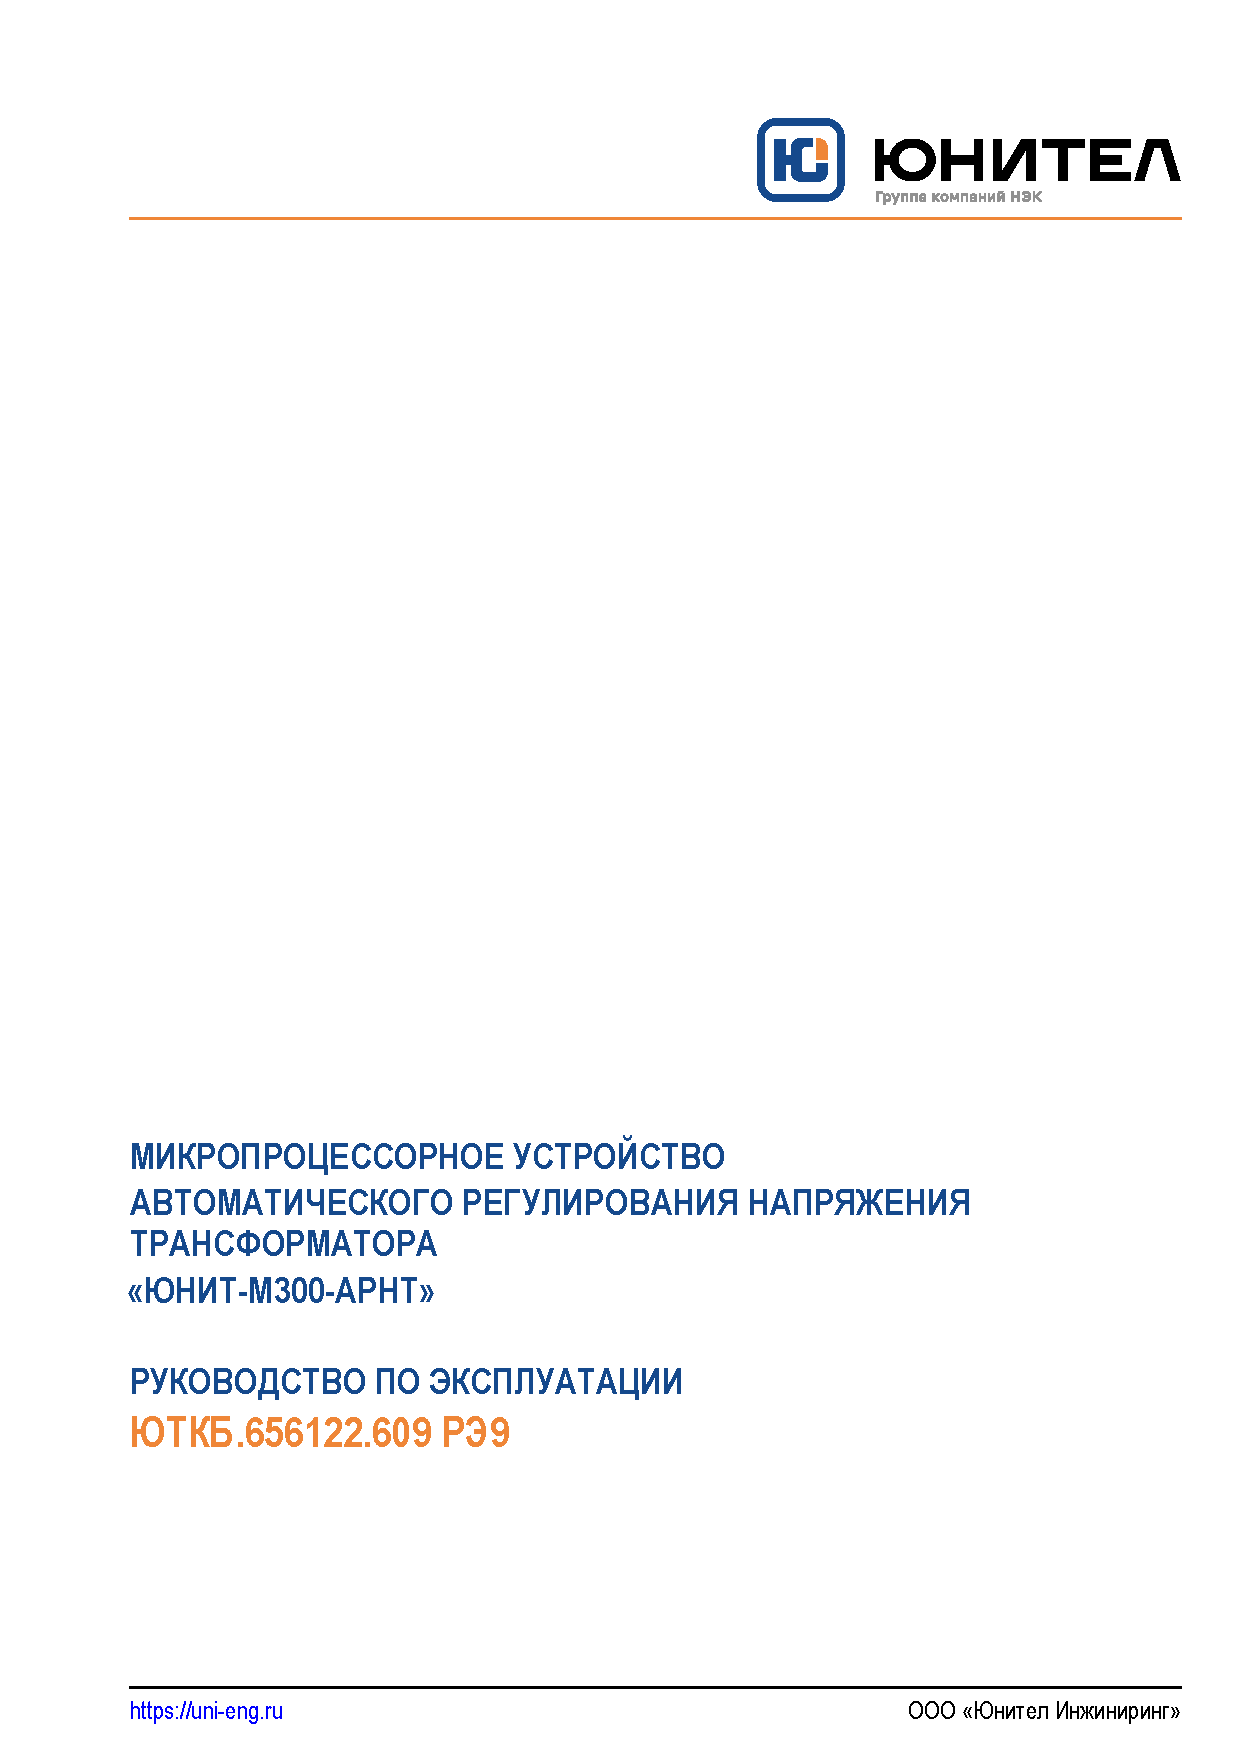
\includepdf[pages={1},width=0.5\textwidth, angle=90]{1.pdf} вставляем и поворачиваем pdf
%\begin{center}
%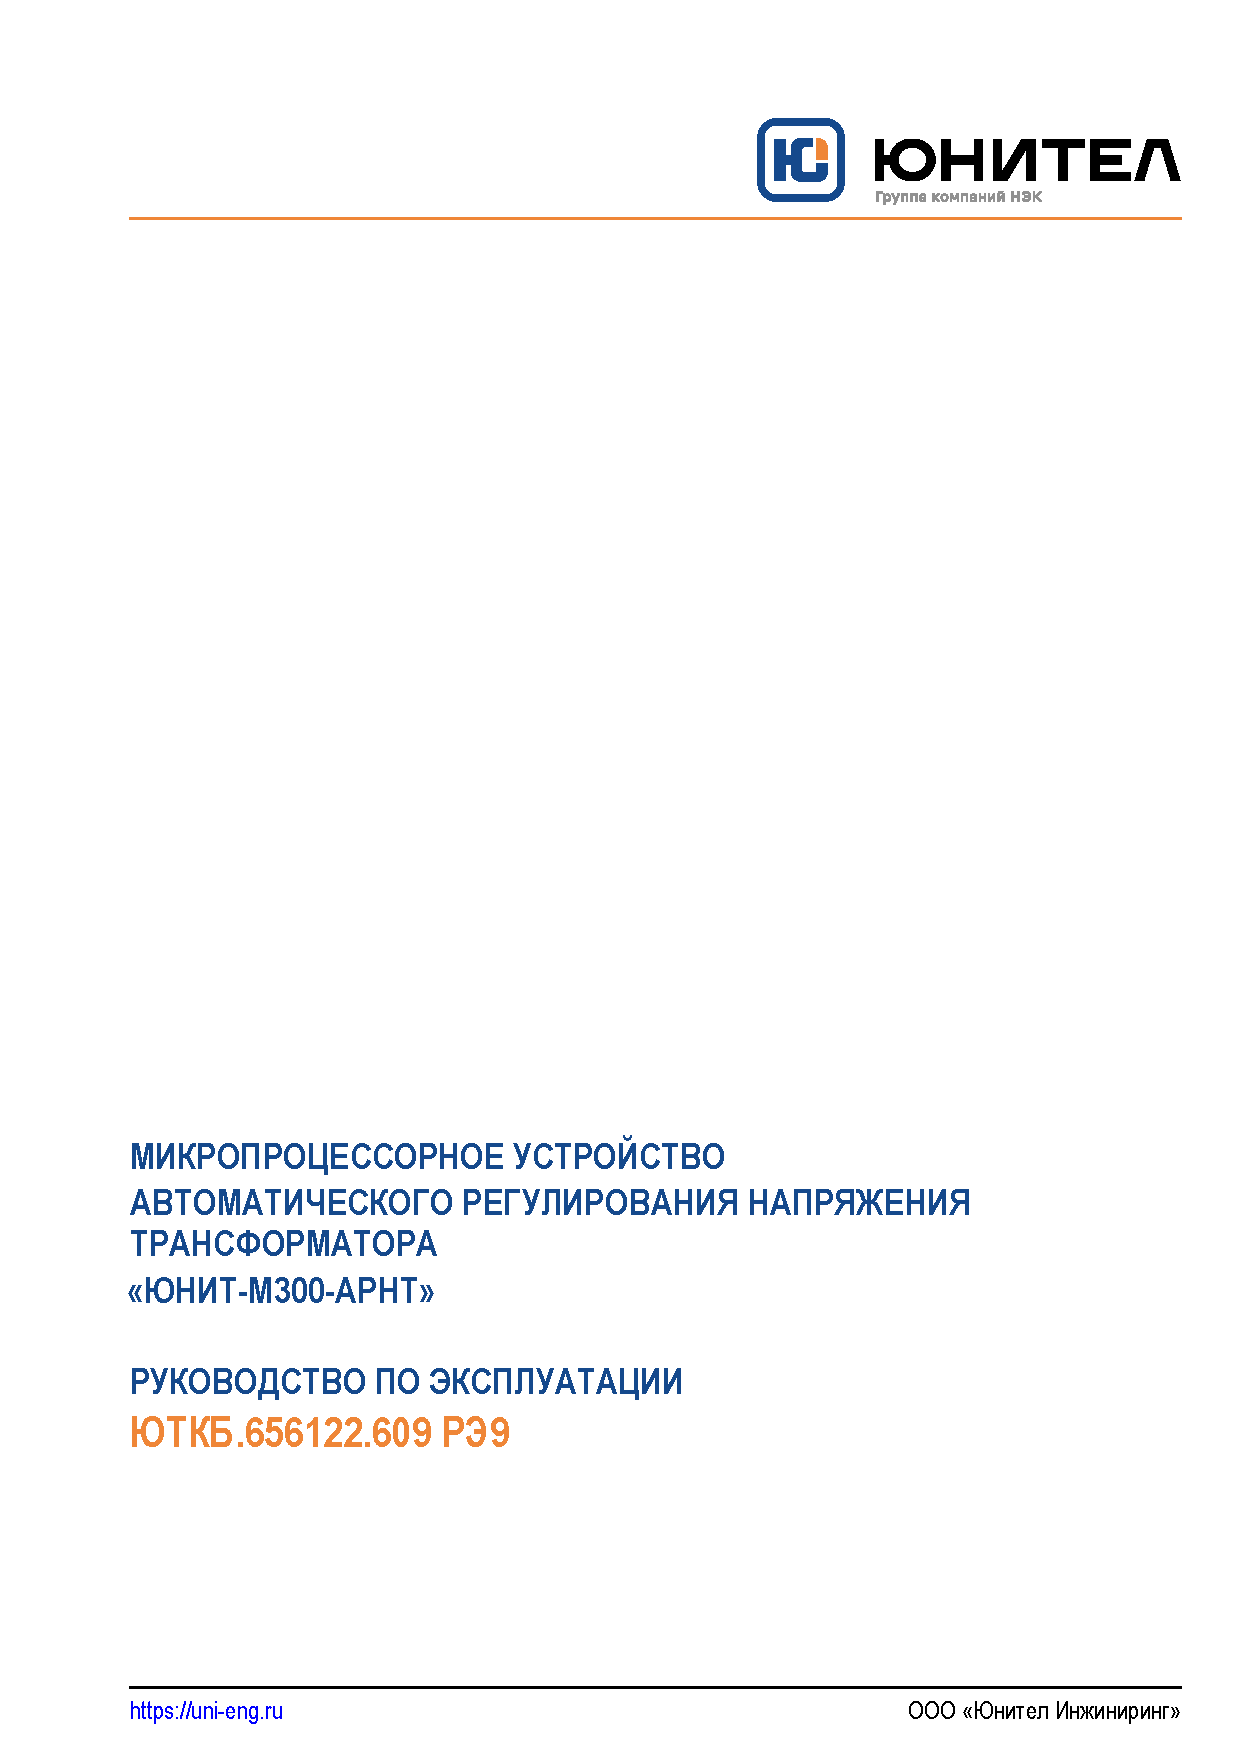
\includegraphics[width=1.4\textwidth]{1.pdf}
%\end{center}

\end{landscape}
\restoregeometry

